\begin{center}
  \textbf{BAB IV} \\[0.5em]
  \textbf{HASIL DAN PEMBAHASAN}
\end{center}

\section*{4.1 Kebutuhan Hardware dan Software}
Hardware maupun Software yang digunakan dalam penelitian ini adalah sebagai berikut:

\begin{itemize}
  \item Hardware:
    \begin{itemize}
      \item CPU: M3
      \item RAM: 18 GB
      \item Storage: 512GB SSD
      \item VGA: M3 GPU
      \item Monitor: 15.6 inch Full HD
      \item Mouse: Wireless
      \item Keyboard: Wireless
    \end{itemize}
  \item Software:
    \begin{itemize}
      \item Operating System: MacOS Sequoia 15.3.2
      \item IDE: Vs Code, Cursor
      \item Database: PostgreSQL
      \item Framework: Laravel
      \item Programming Language: PHP, JavaScript, HTML, CSS, SQL
    \end{itemize}
\end{itemize}

\section*{4.2 Implementasi}

Langkah berikutnya setelah melakukan perancangan sistem adalah implementasi sistem dalam pengkodean. 
Berikut adalah hasil implementasi dari sistem yang telah dirancang.

\subsection*{4.2.1 Tampilan UI Register}
halaman register digunakan untuk membuat akun baru pada sistem.
\begin{center}
  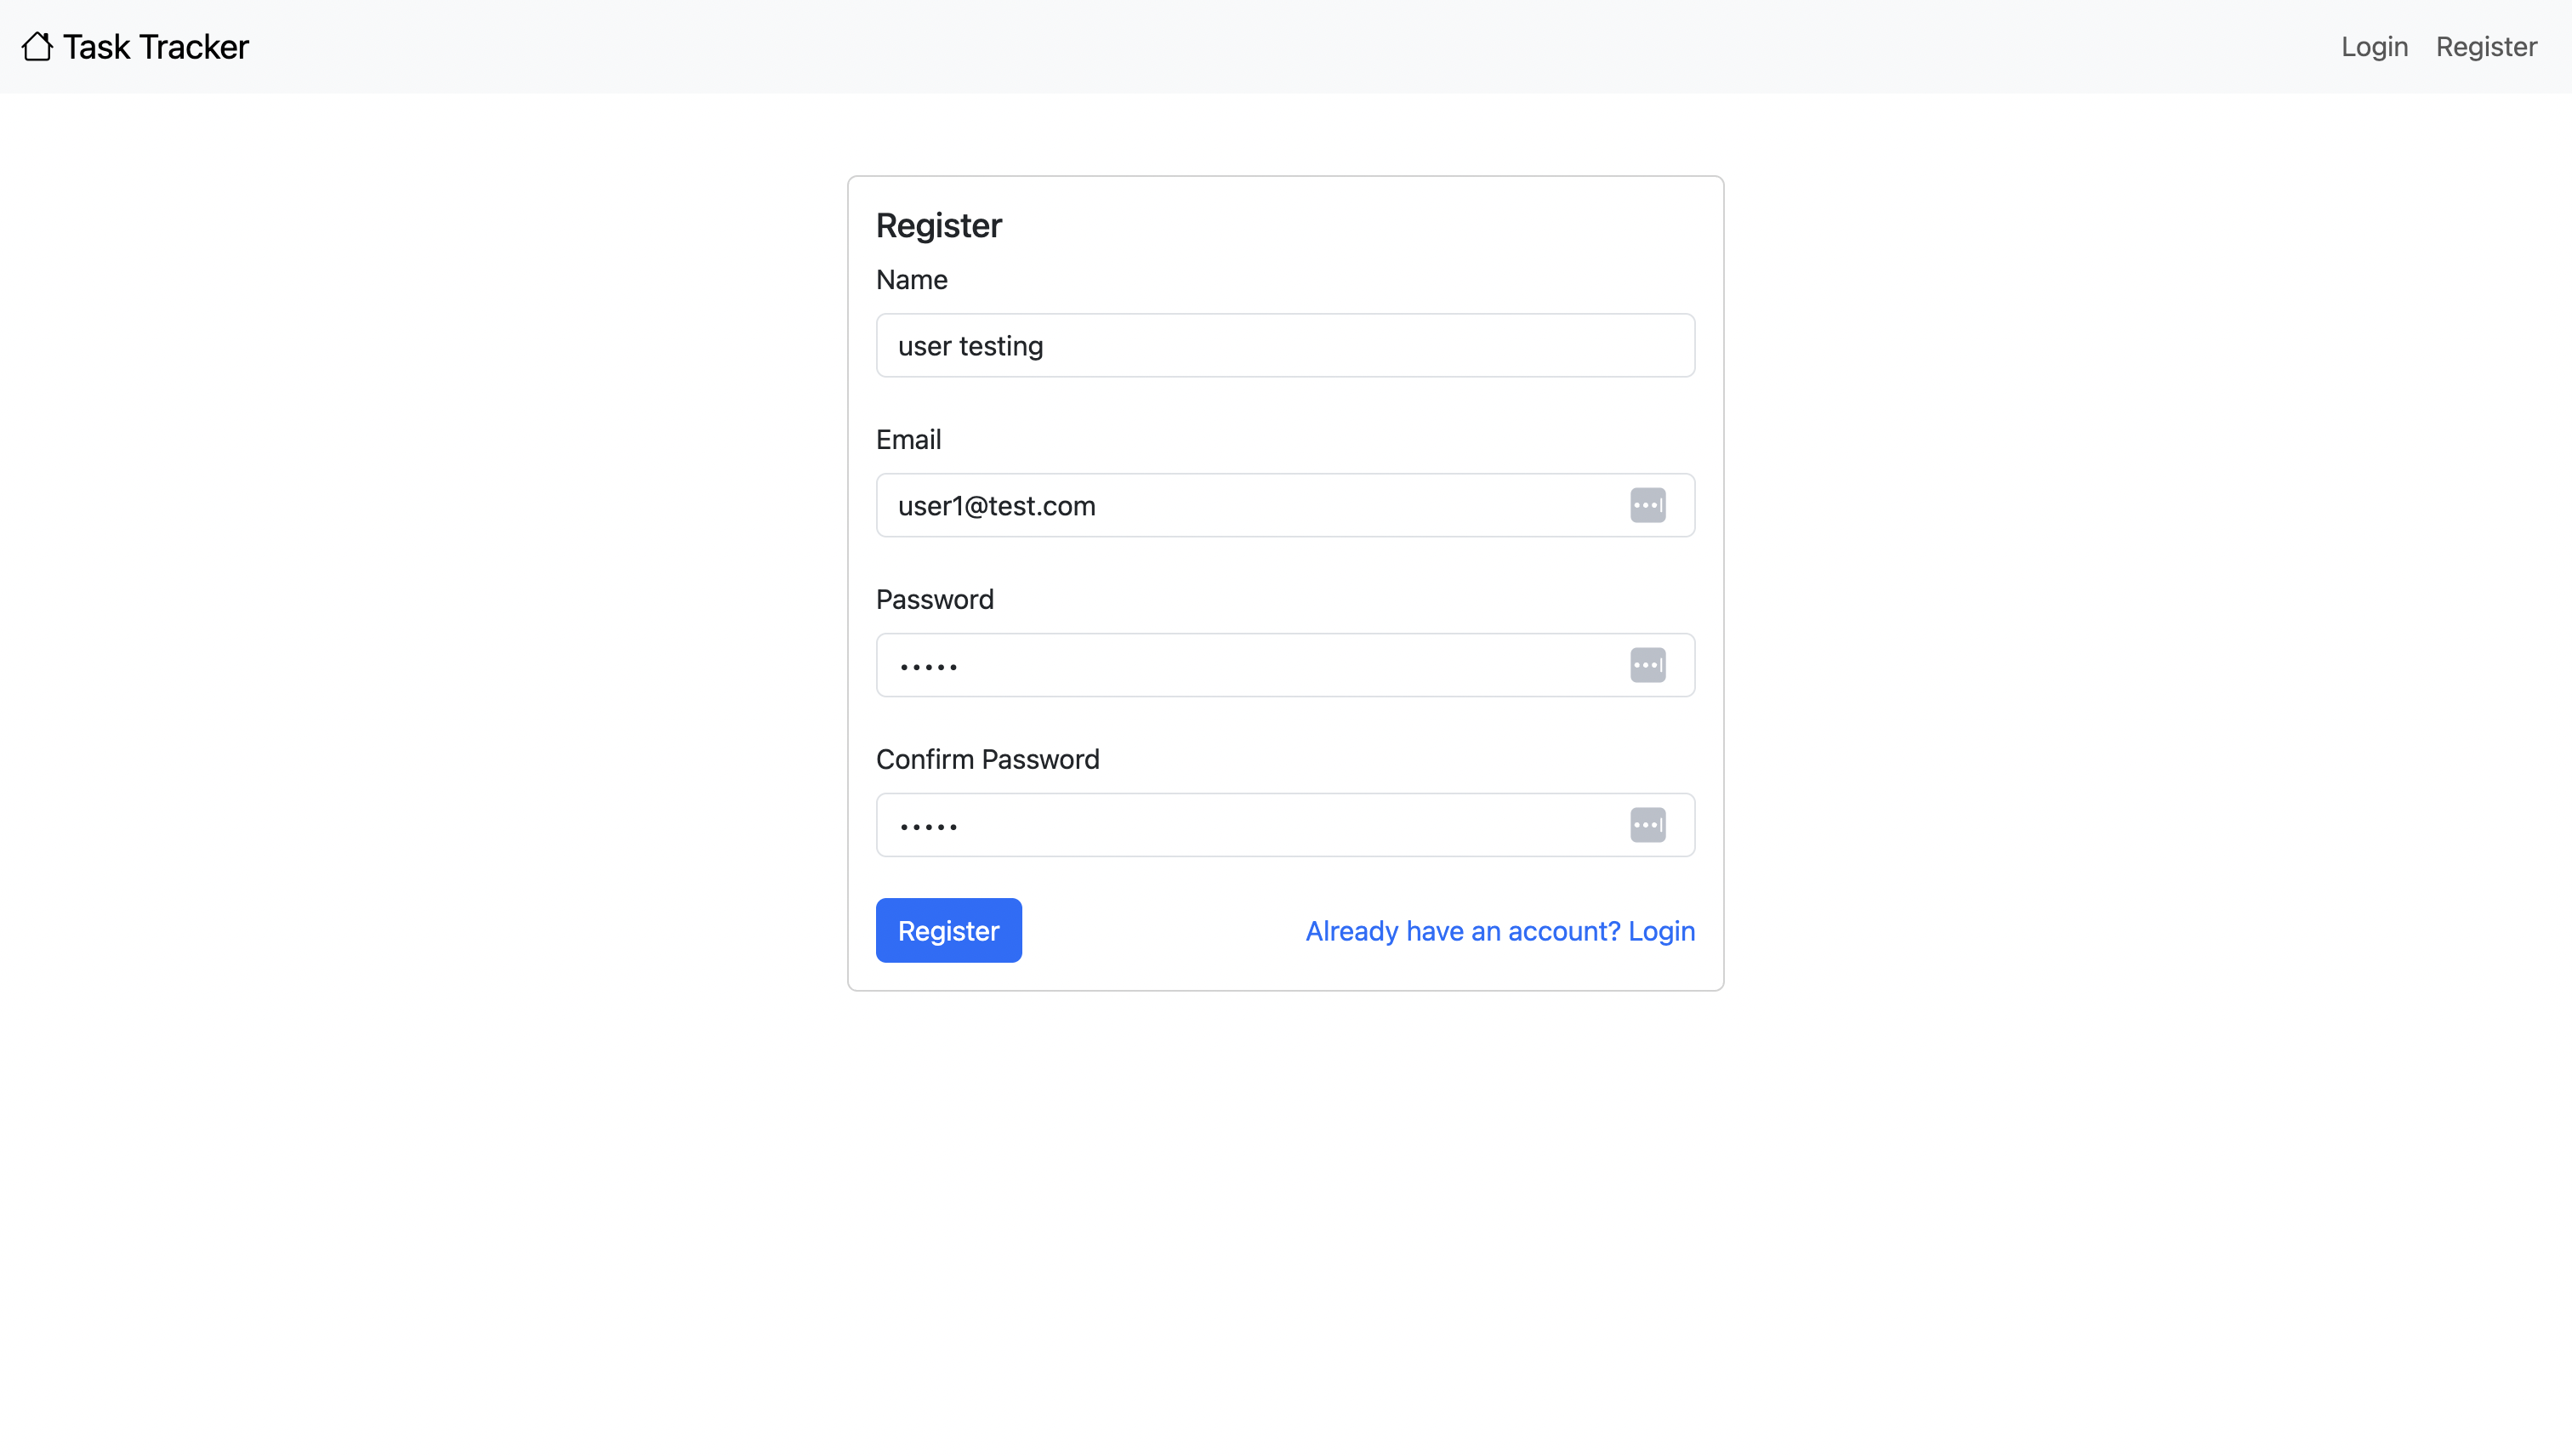
\includegraphics[width=1\textwidth]{assets/ui/register_filled.png}
  \captionof{figure}{Tampilan UI Register}
\end{center}


\subsection*{4.2.2 Tampilan UI Login}
halaman login digunakan untuk masuk ke dalam sistem.
\begin{center}
  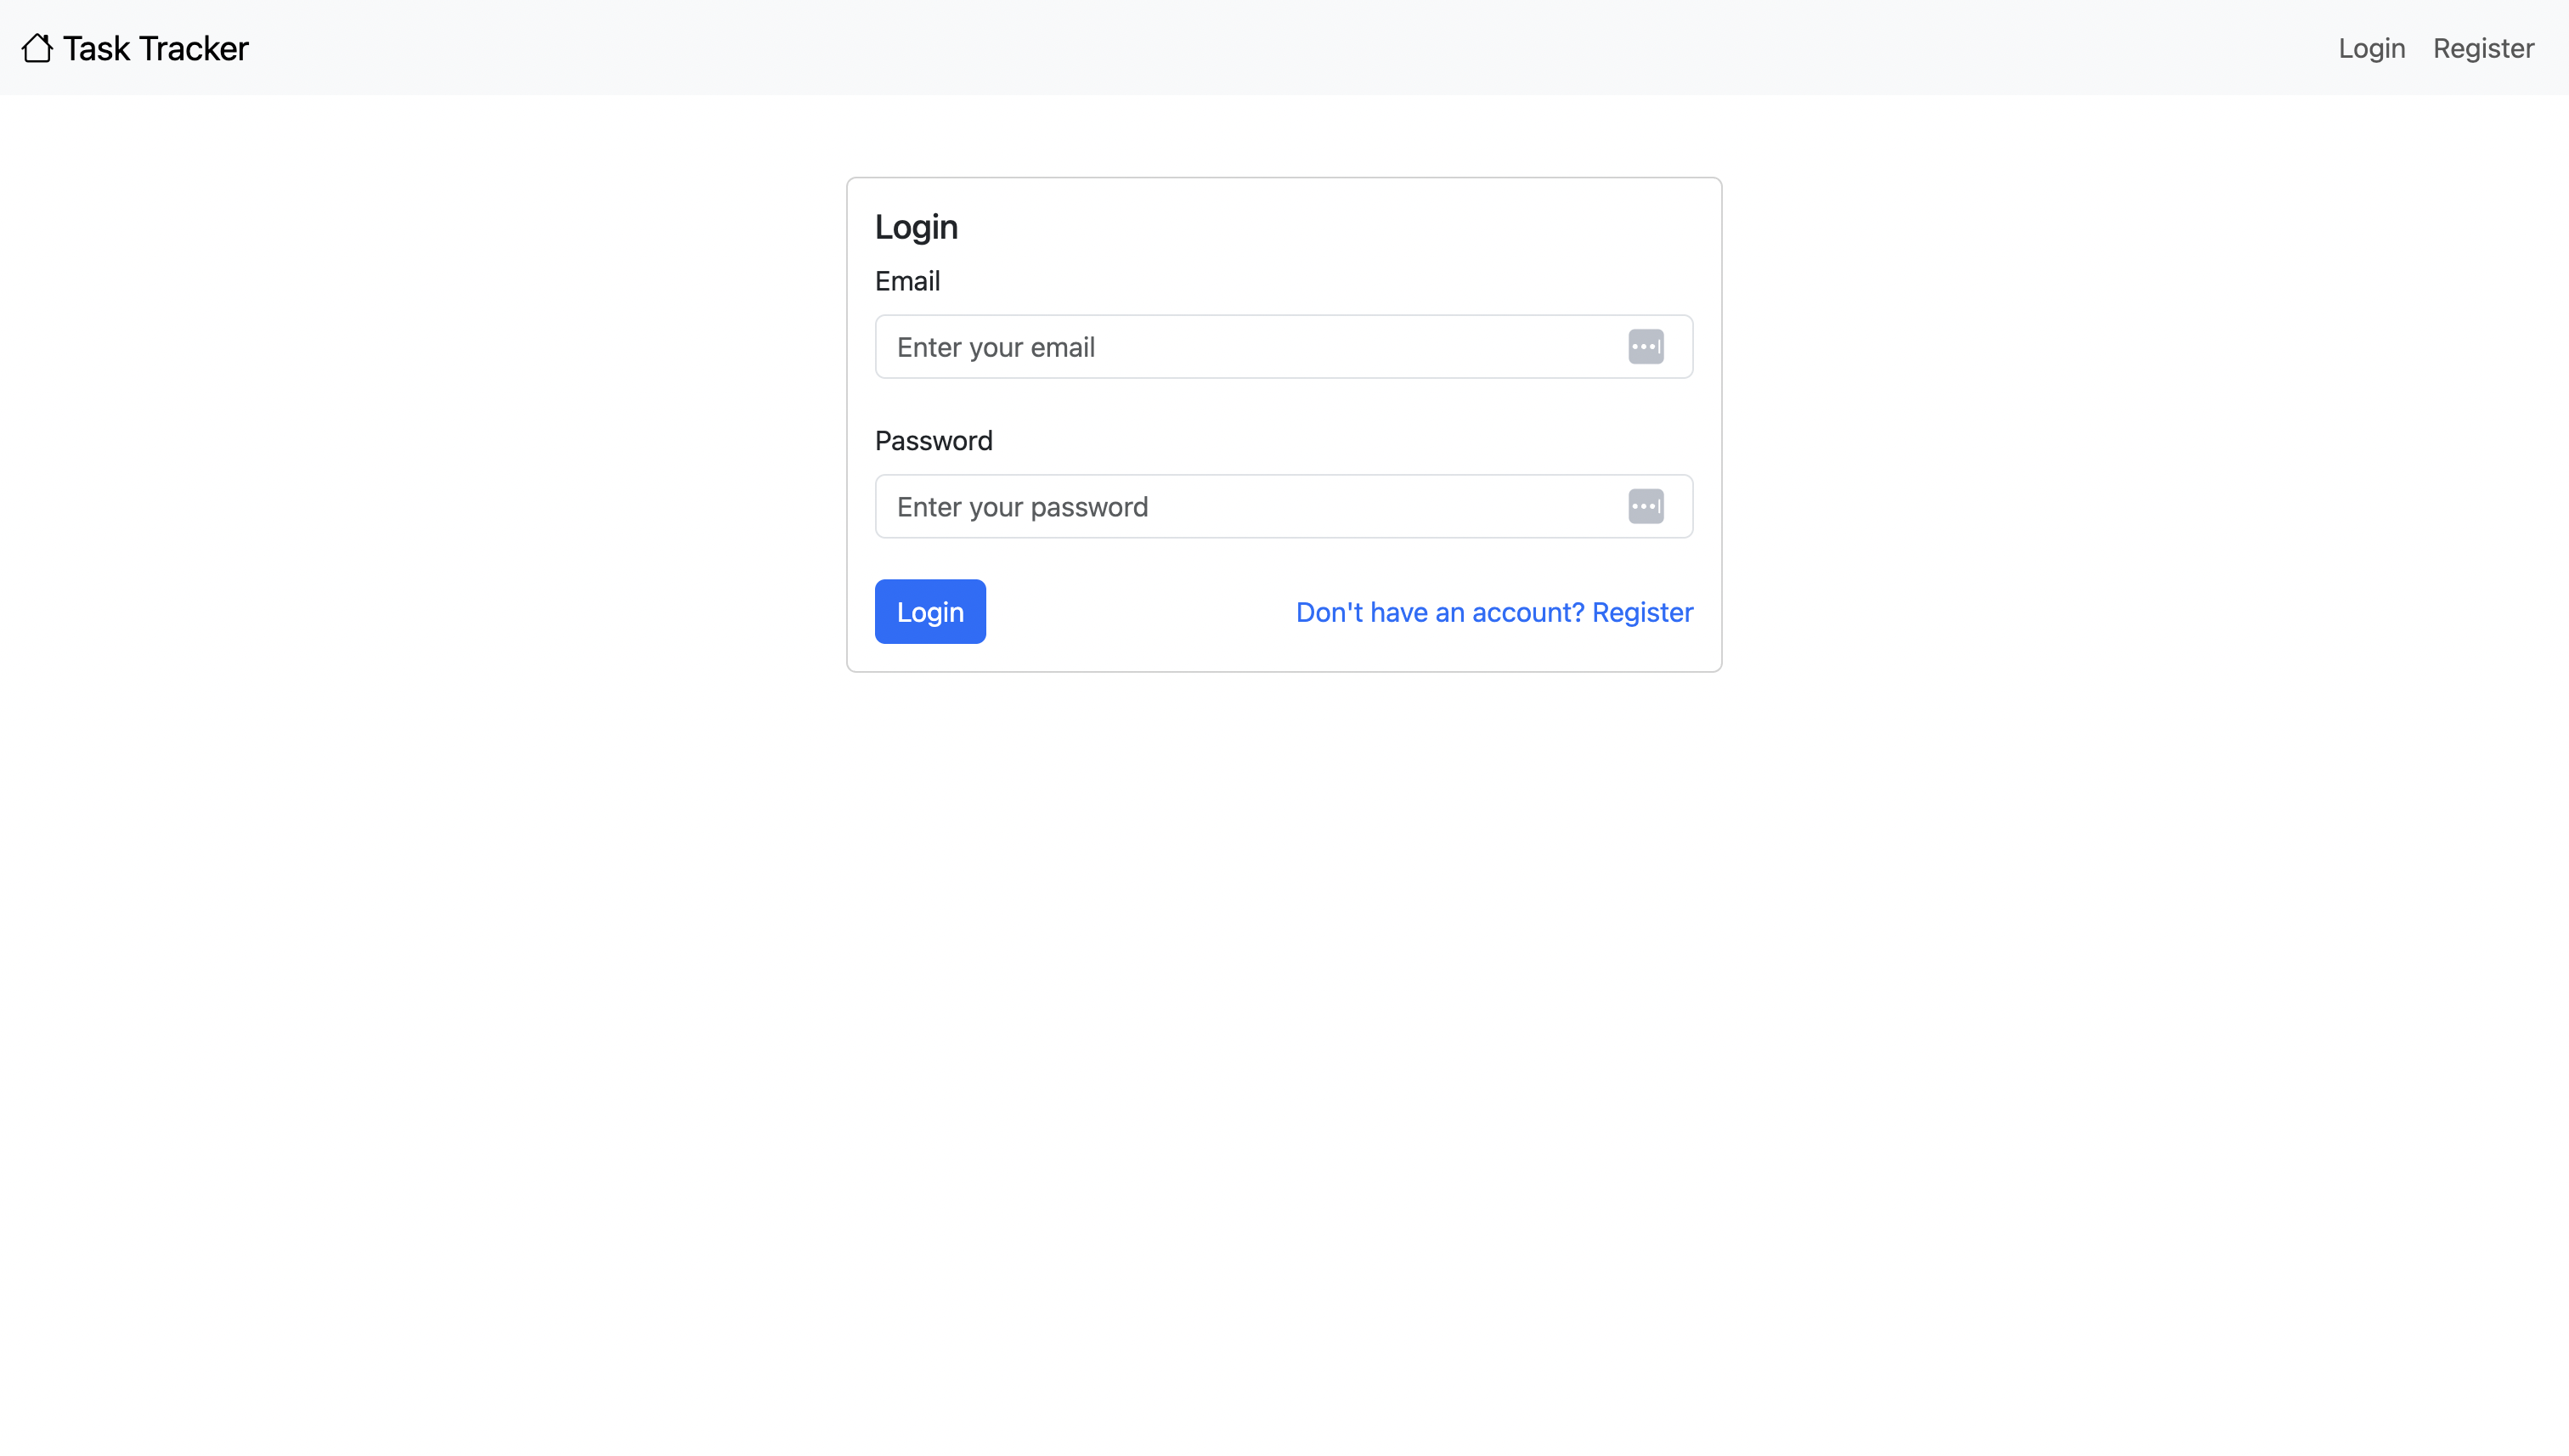
\includegraphics[width=1\textwidth]{assets/ui/login.png}
  \captionof{figure}{Tampilan UI Login}
\end{center}

\subsection*{4.2.3 Tampilan UI Dashboard}
halaman dashboard digunakan untuk menampilkan informasi terkait akun yang sedang login.
\begin{center}
  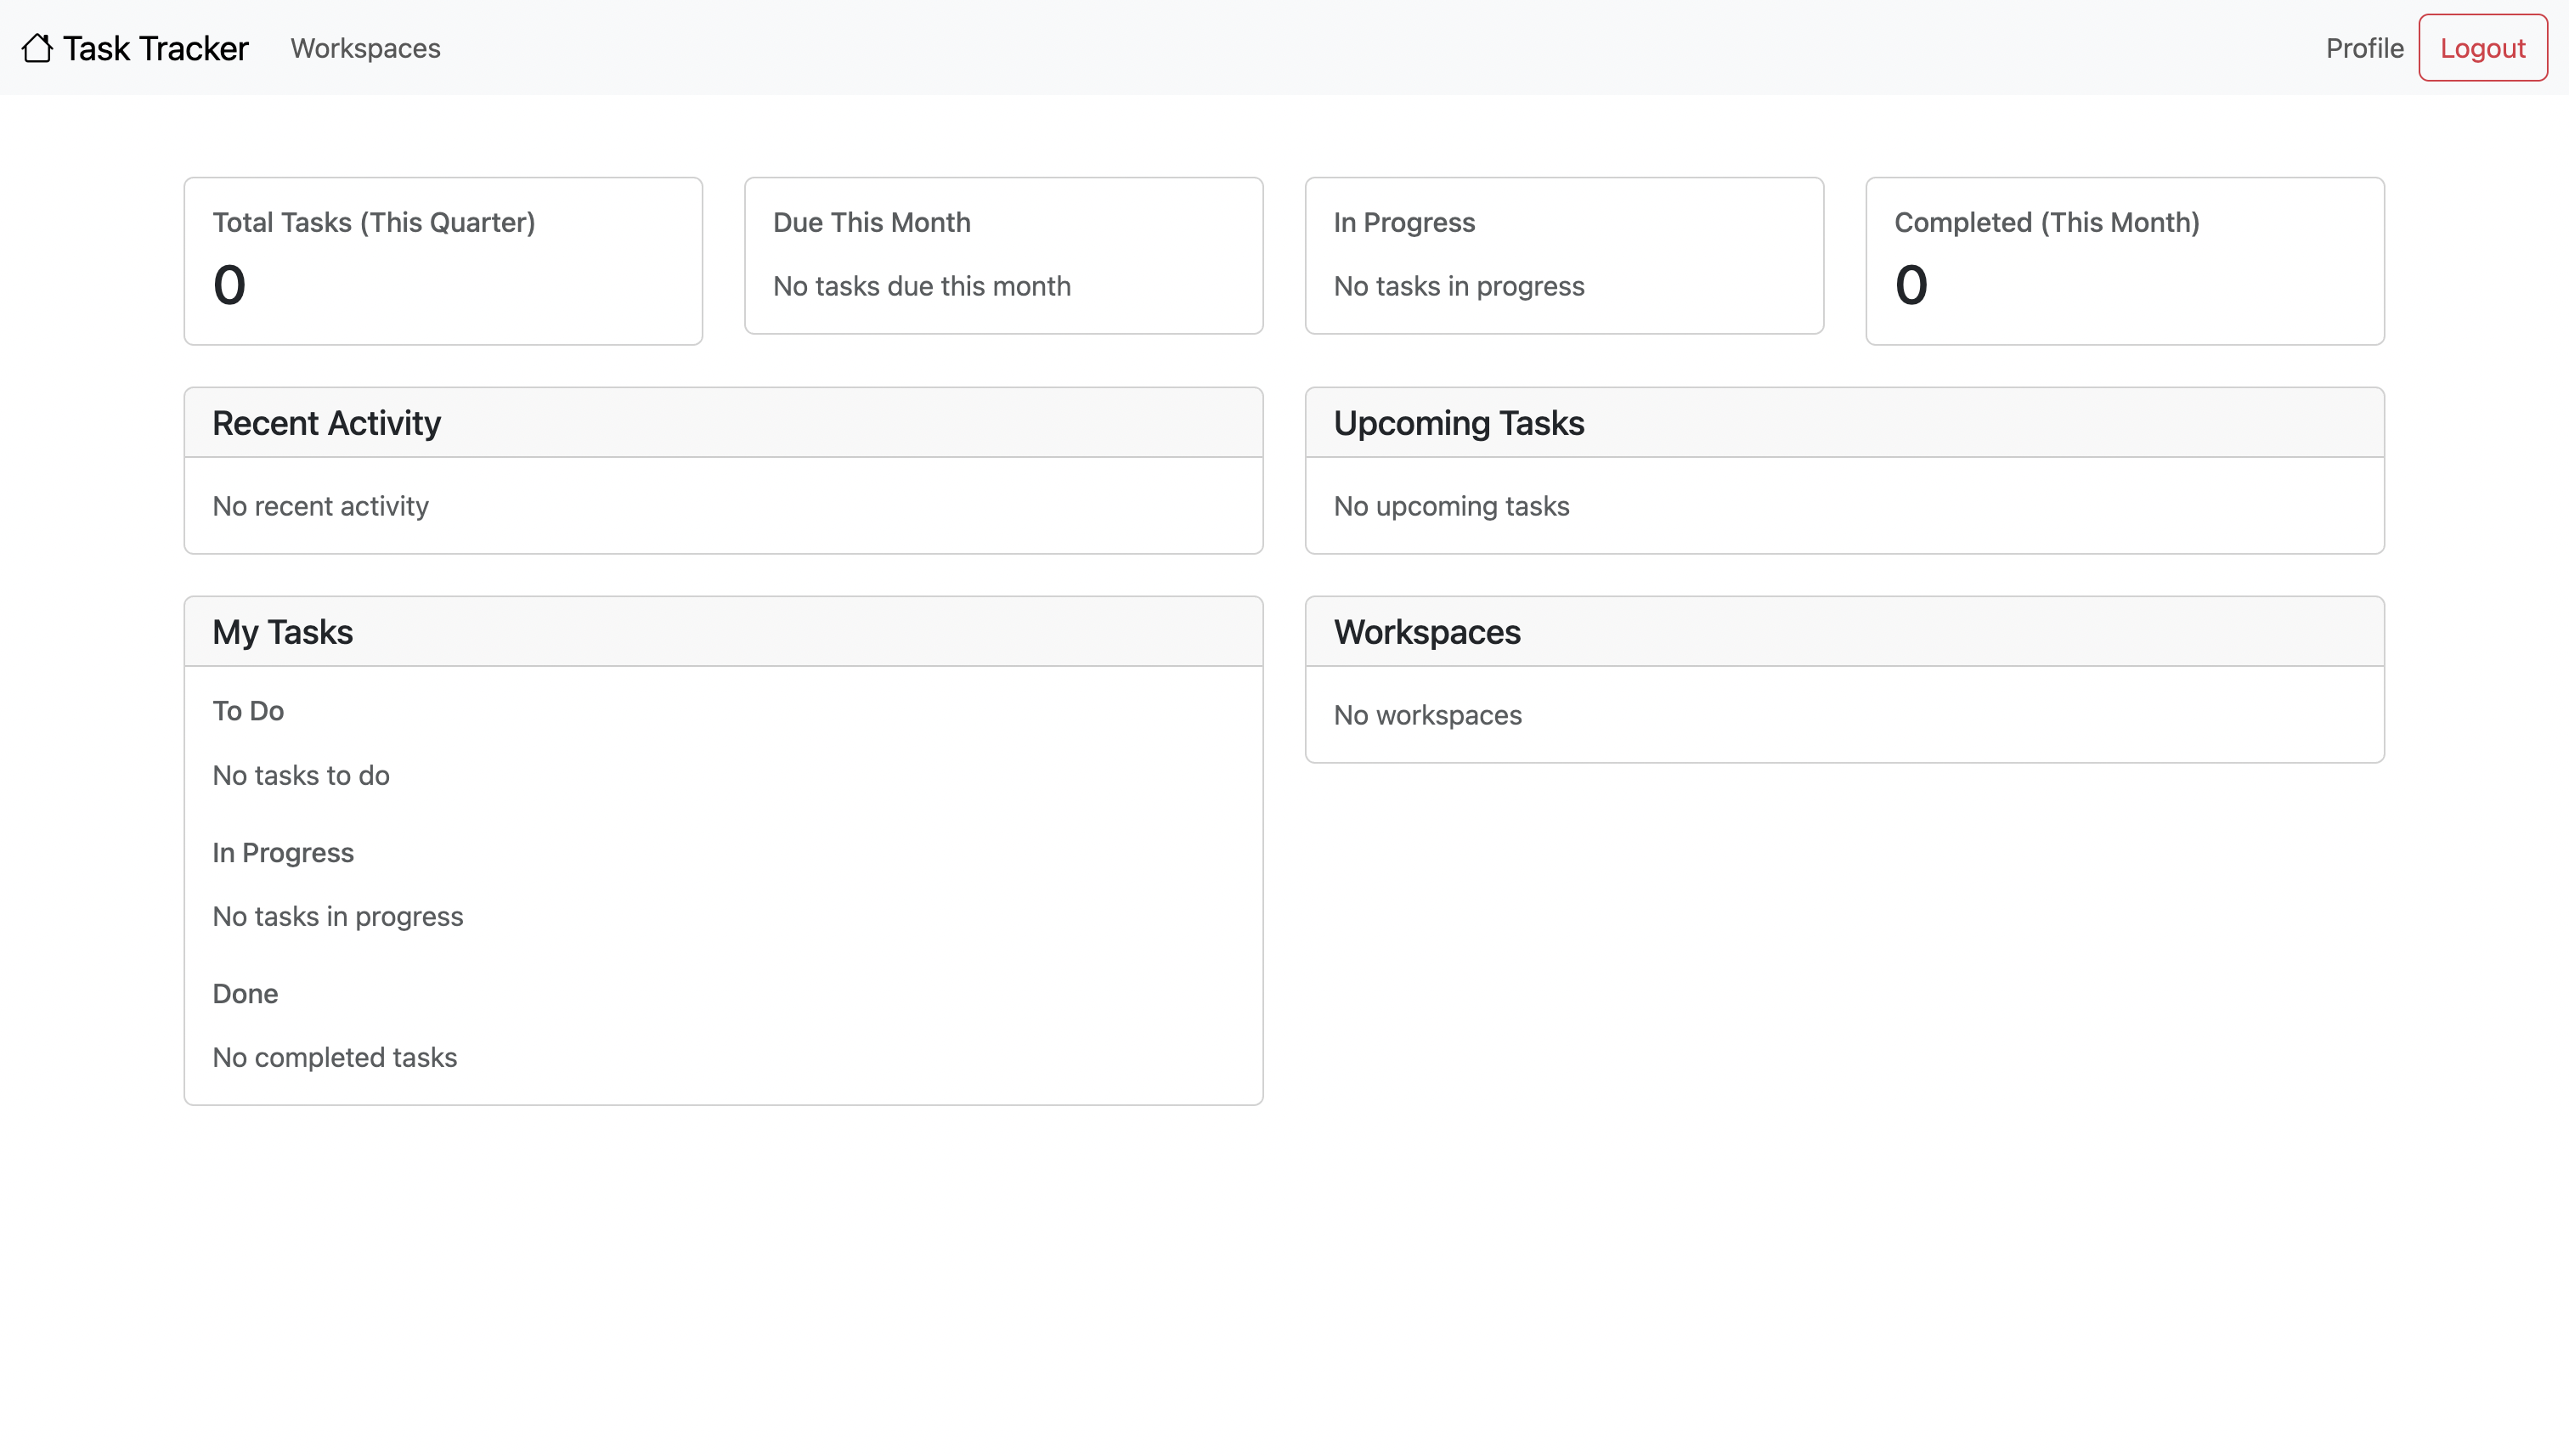
\includegraphics[width=1\textwidth]{assets/ui/empty_dashboard.png}
  \captionof{figure}{Tampilan UI Dashboard Kosong}
\end{center}
\begin{center}
  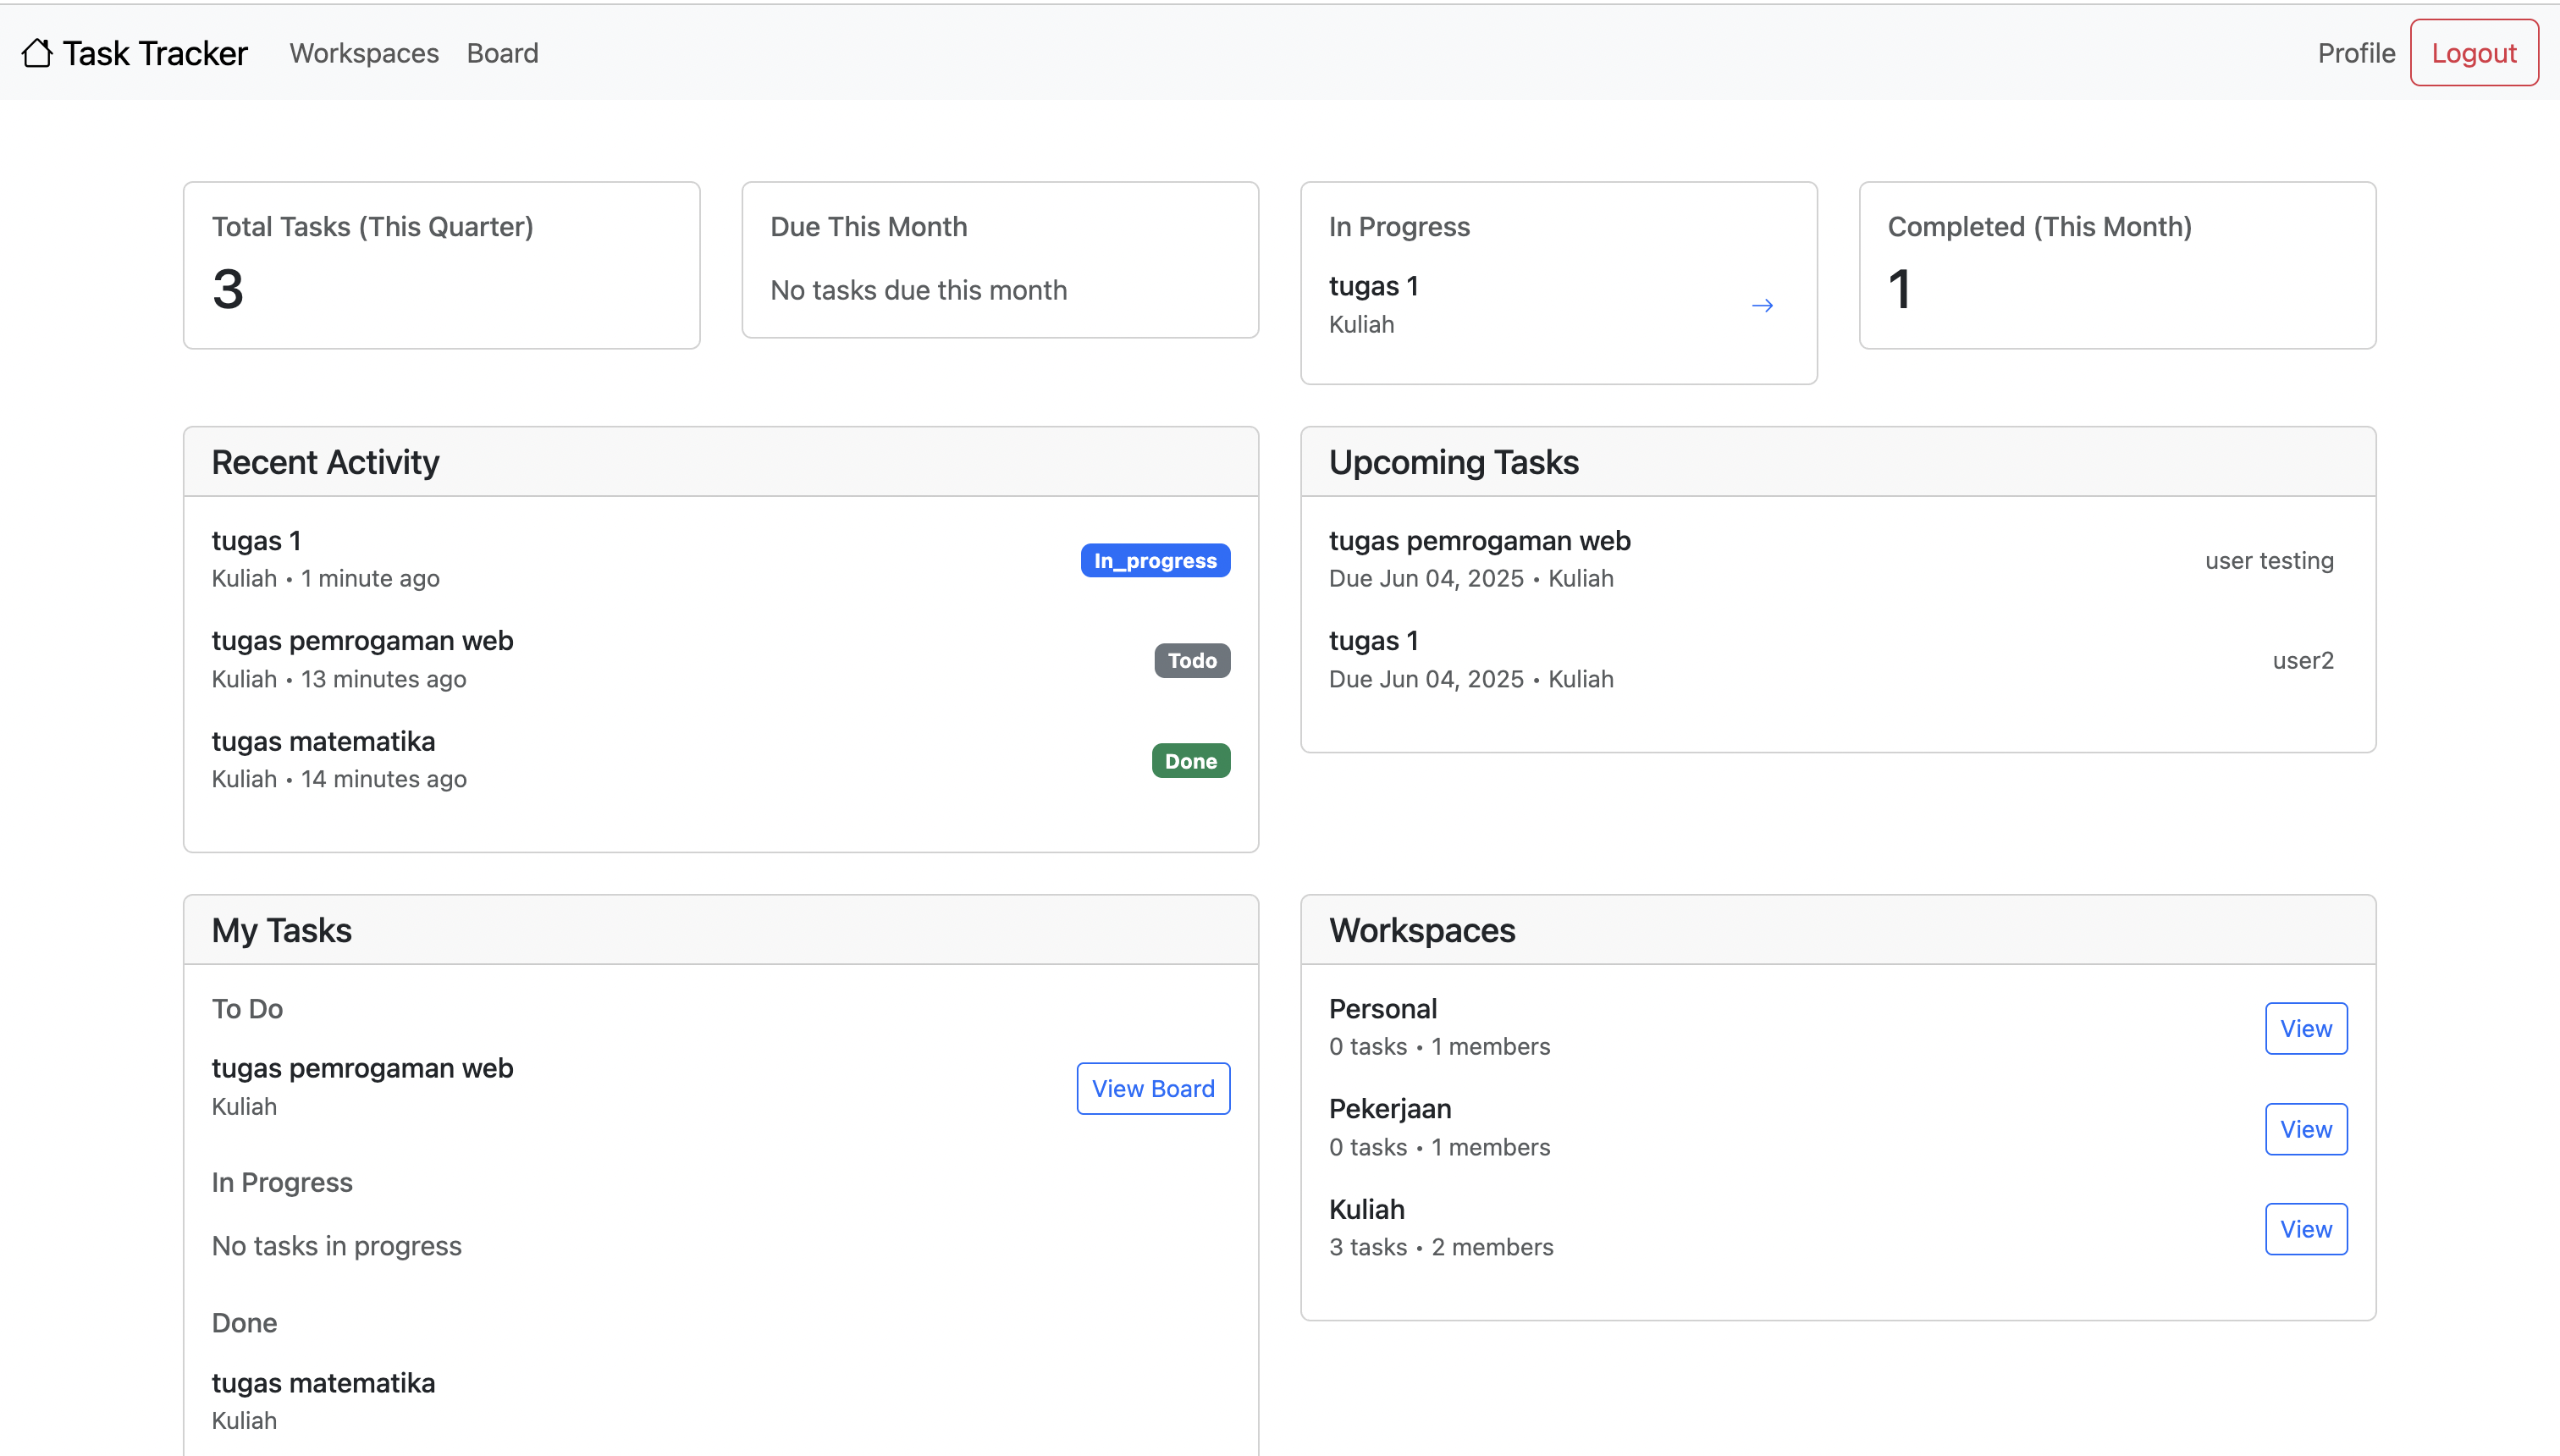
\includegraphics[width=1\textwidth]{assets/ui/user_dashboard_filled.png}
  \captionof{figure}{Tampilan UI Dashboard Terisi}
\end{center}

\subsection*{4.2.4 Tampilan UI Profile}
halaman profile digunakan untuk menampilkan informasi terkait akun yang sedang login.
halman ini juga digunakan untuk mengubah informasi akun yang sedang login, seperti nama dan password.
\begin{center}
  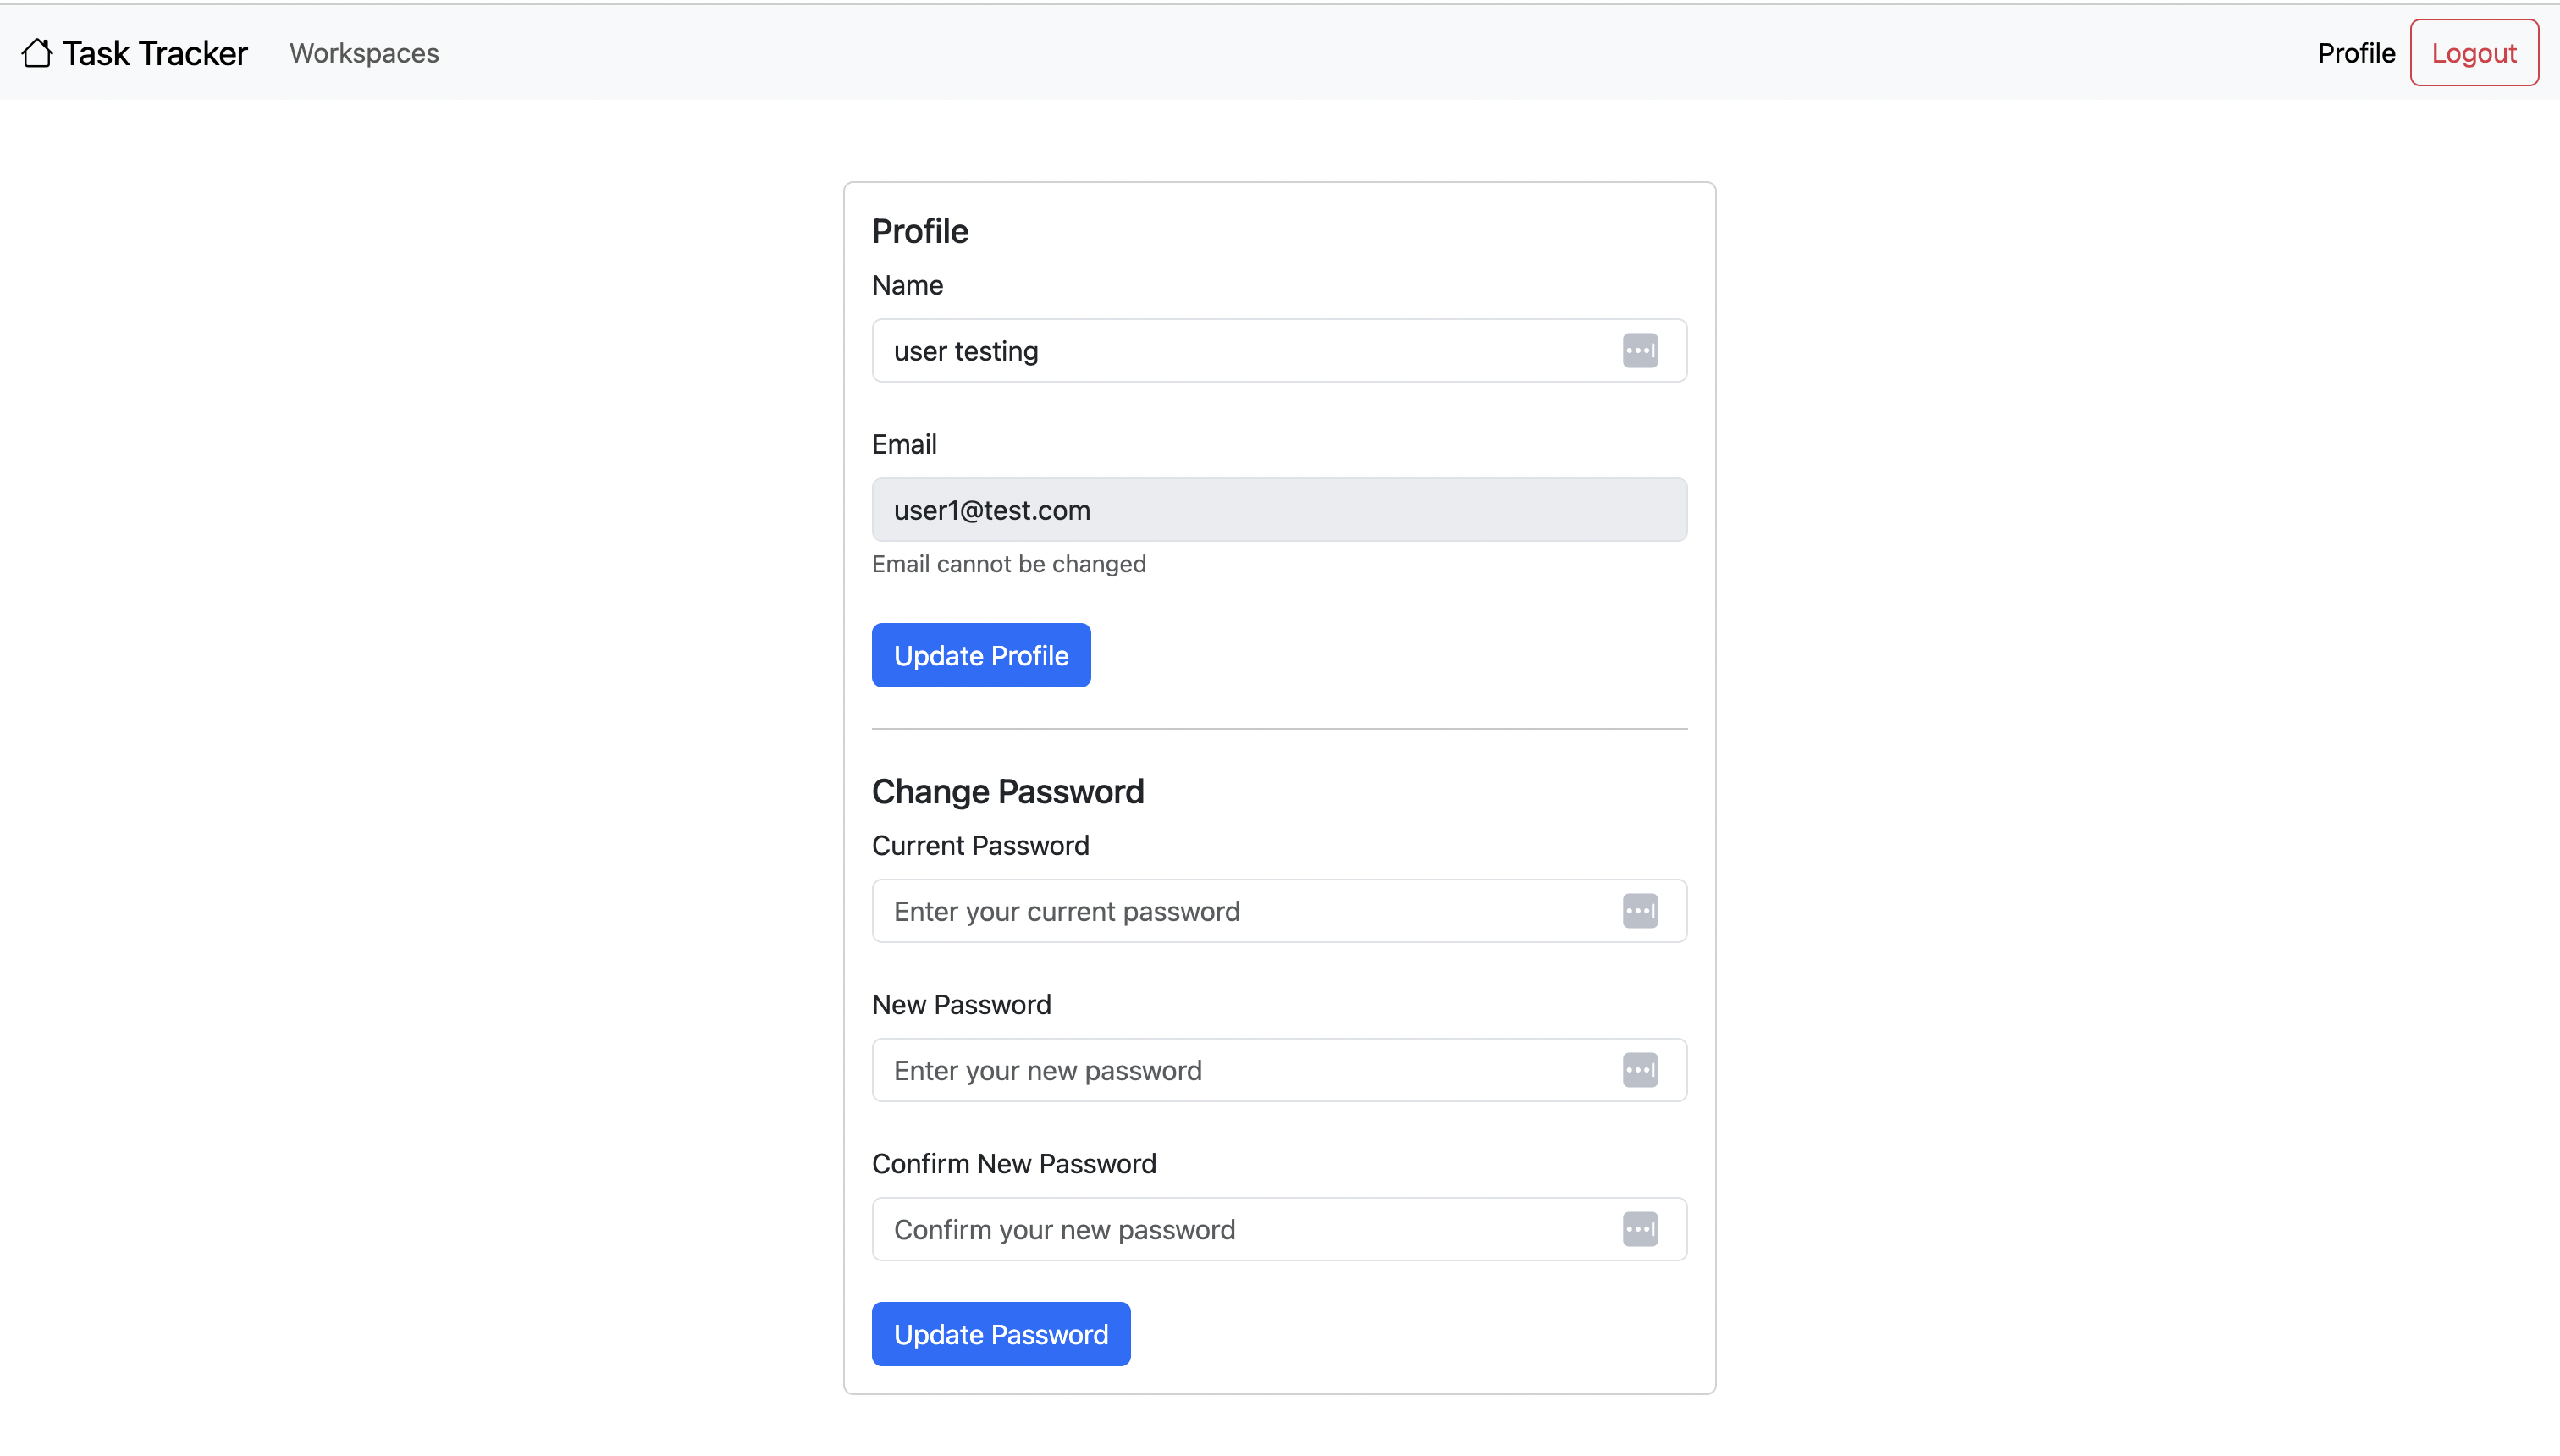
\includegraphics[width=1\textwidth]{assets/ui/edit_profile.png}
  \captionof{figure}{Tampilan UI Profile}
\end{center}



\subsection*{4.2.5 Tampilan UI Workspace}
halaman workspace digunakan untuk manajemen workspace. 
seperti membuat workspace baru, mengubah nama workspace, dan menghapus workspace.
\begin{center}
  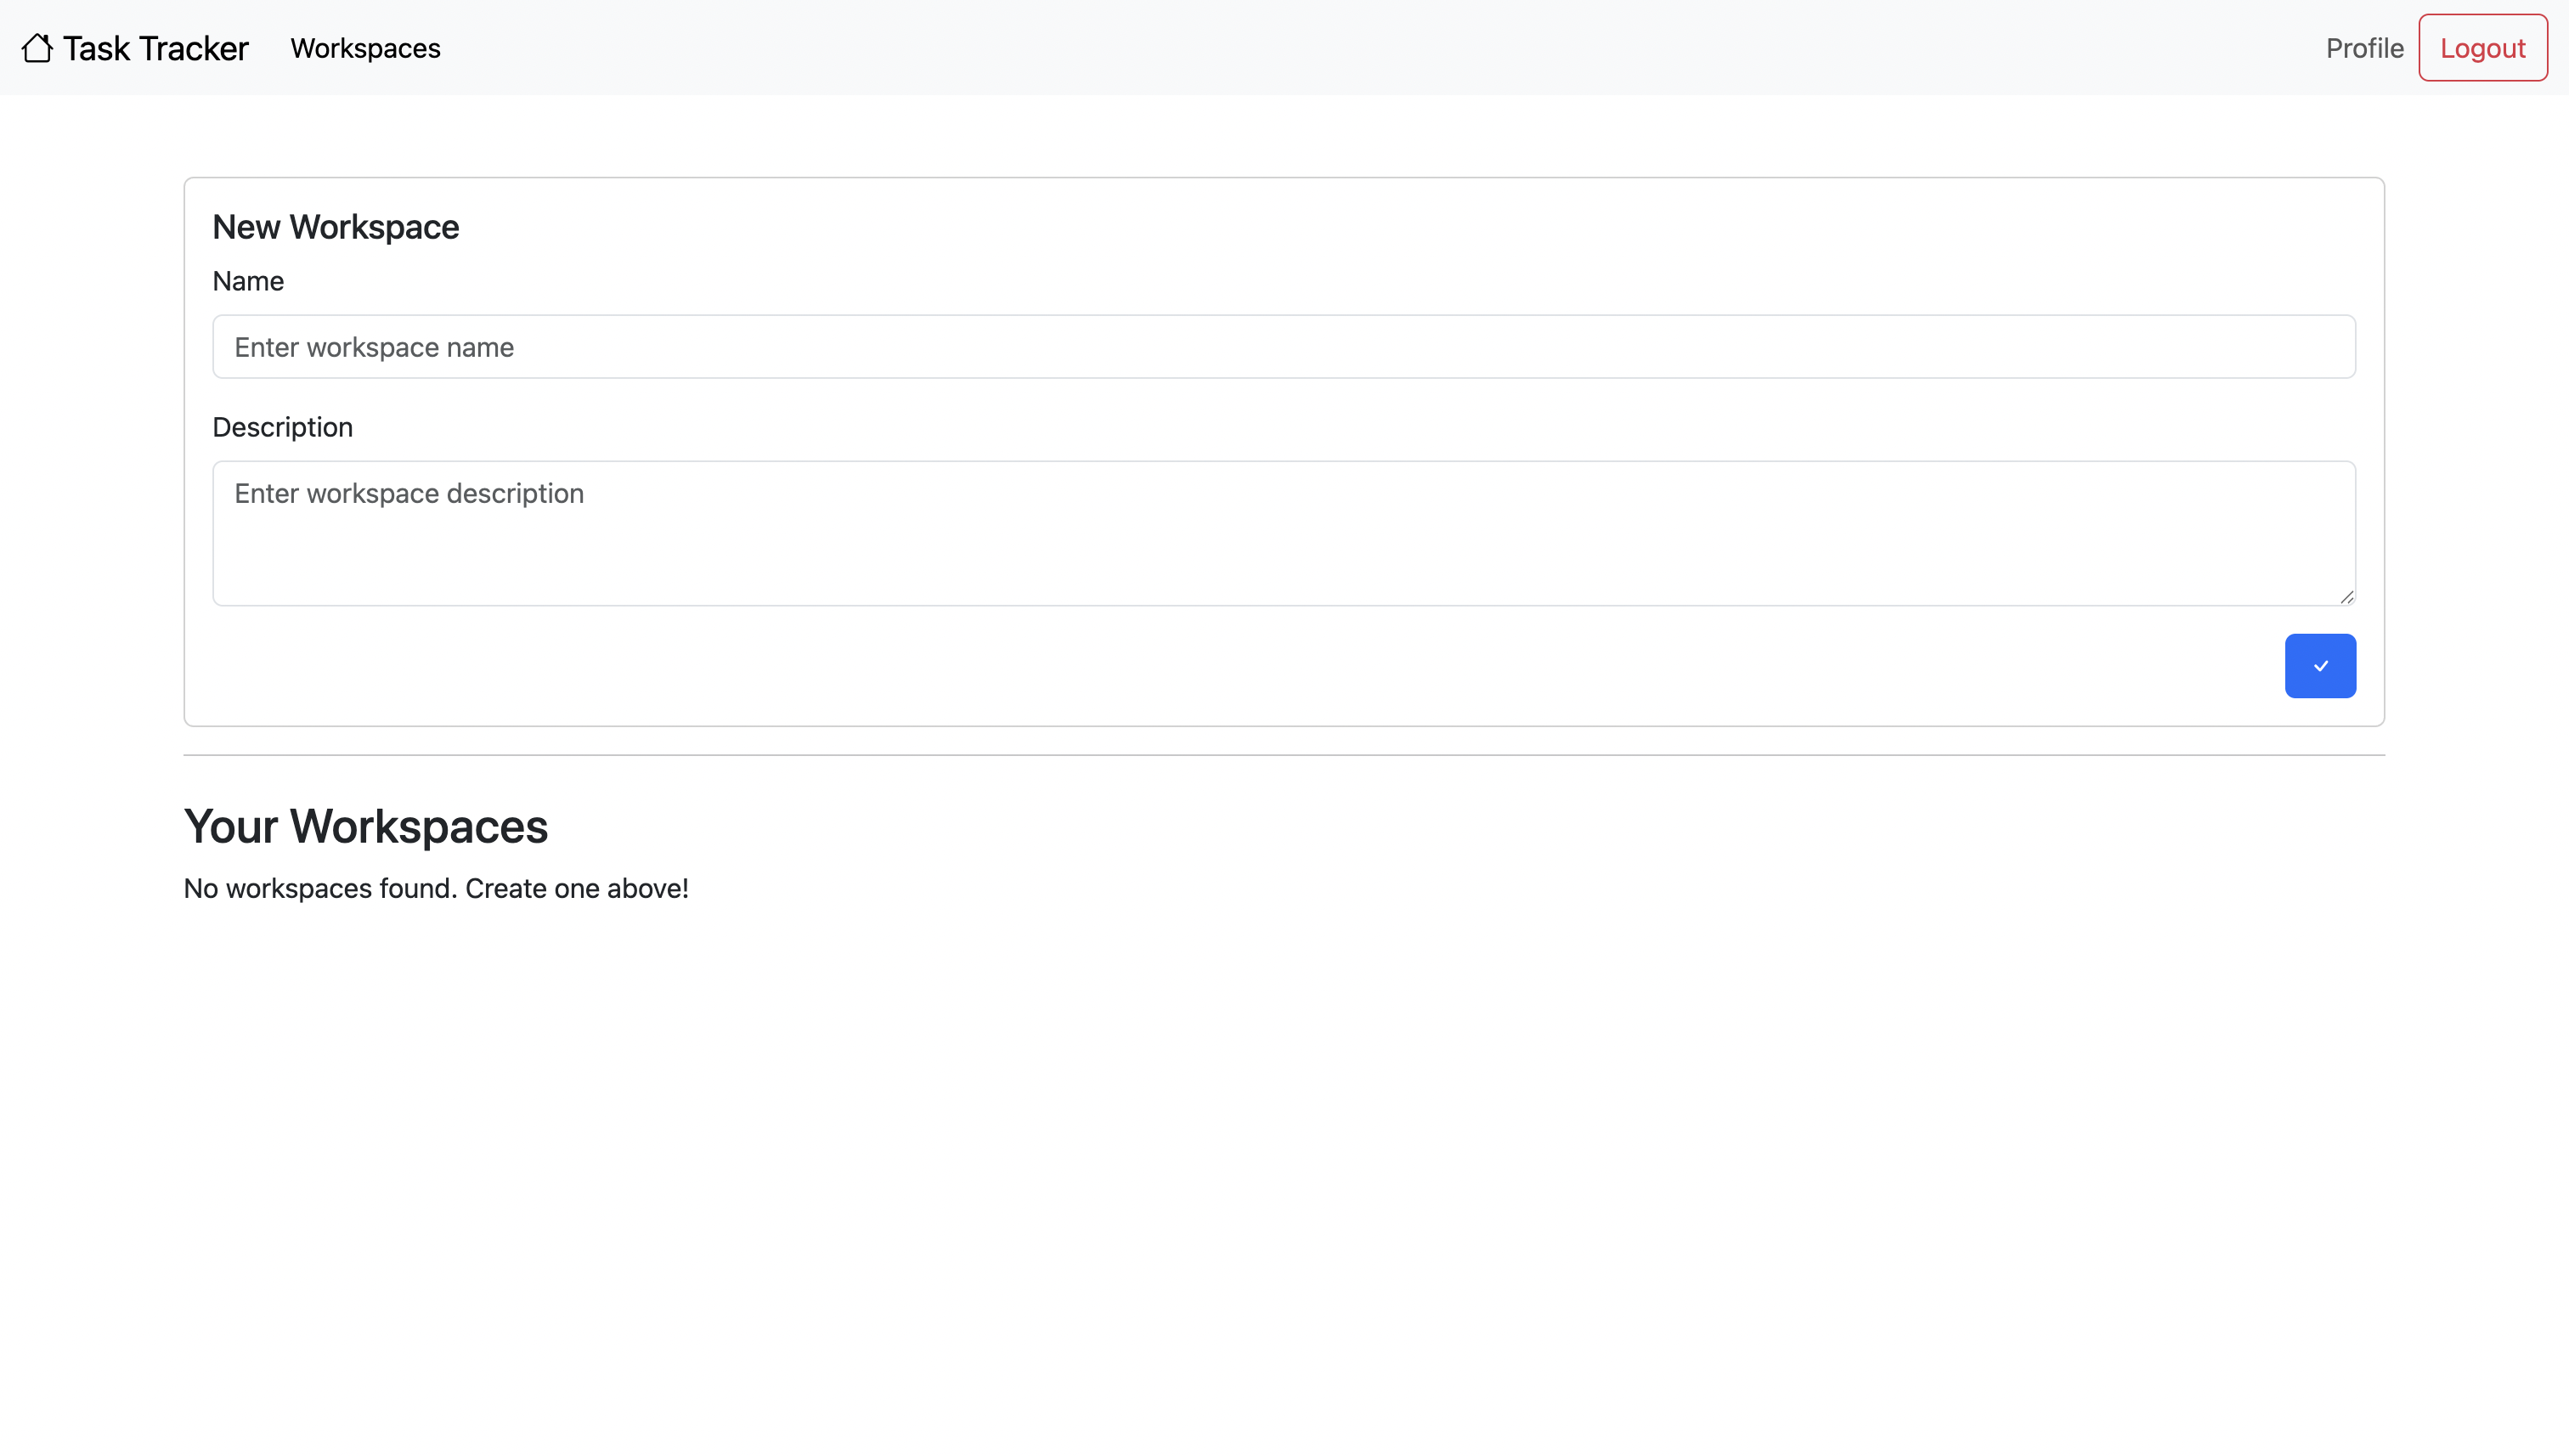
\includegraphics[width=1\textwidth]{assets/ui/workspace_empty.png}
  \captionof{figure}{Tampilan UI Workspace Kosong}
\end{center}
\begin{center}
  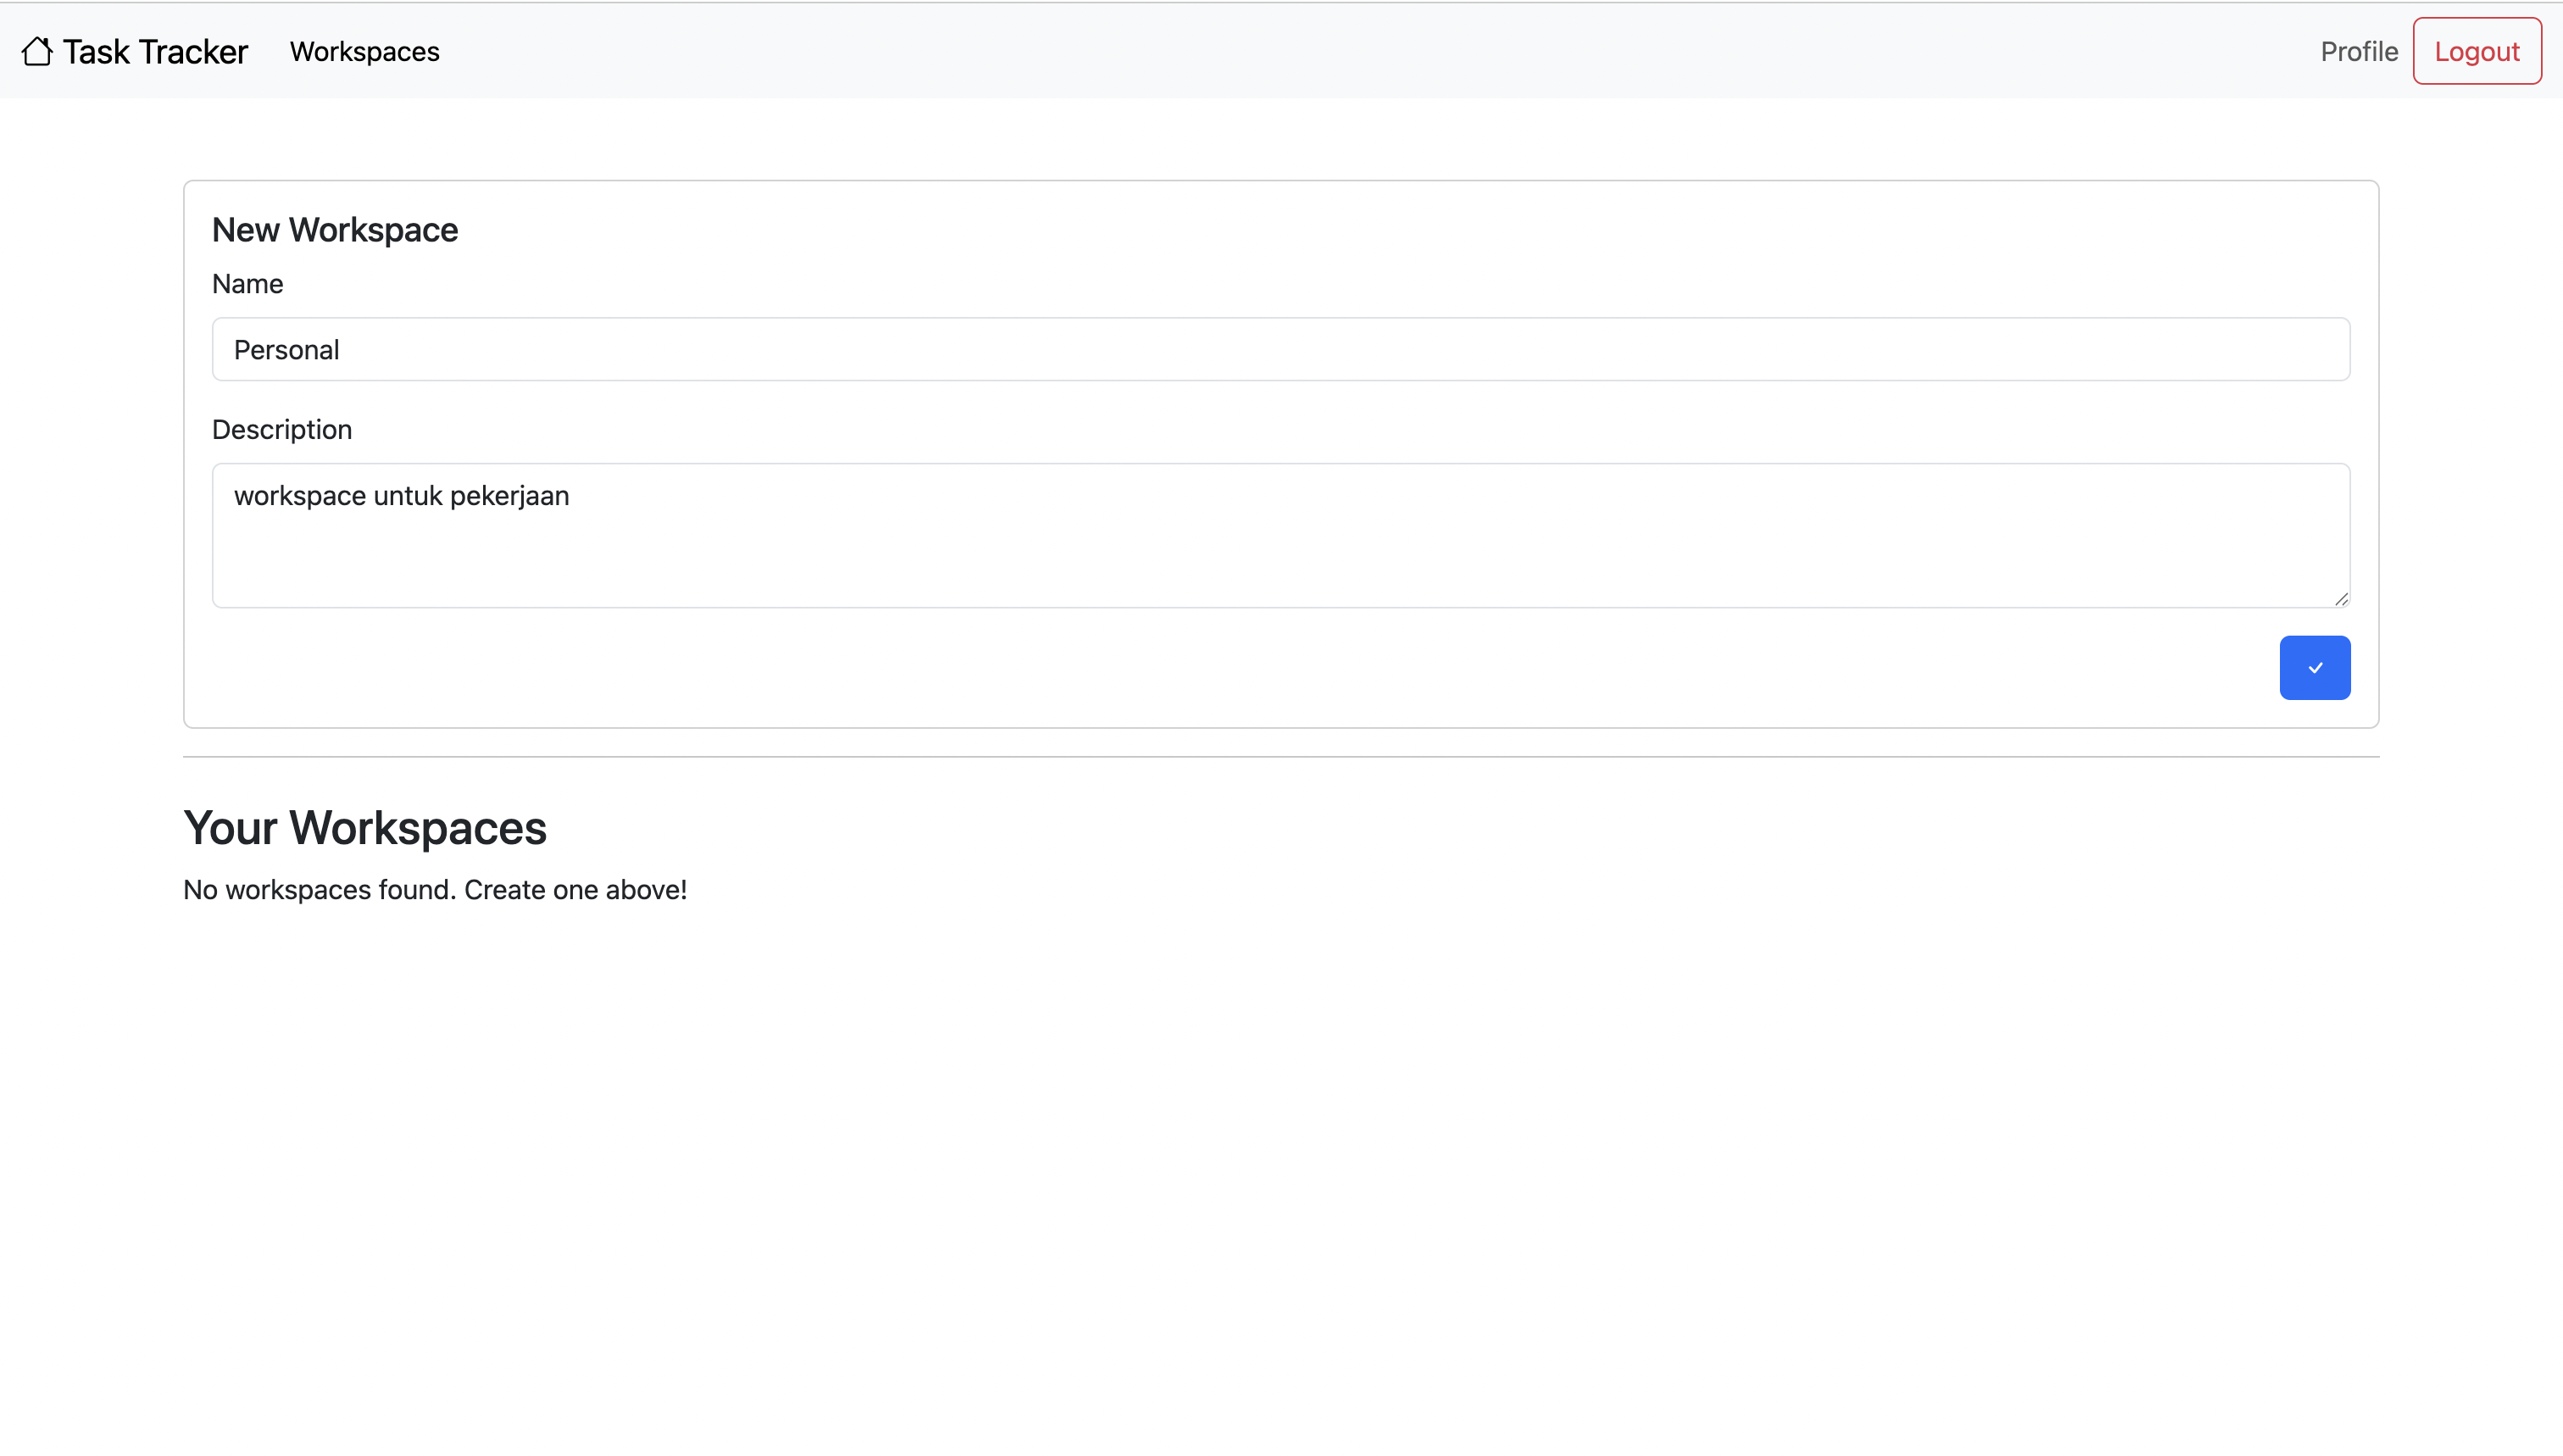
\includegraphics[width=1\textwidth]{assets/ui/workspace_create_filled.png}
  \captionof{figure}{Tampilan UI Workspace dengan Form Create Workspace Terisi}
\end{center}
\begin{center}
  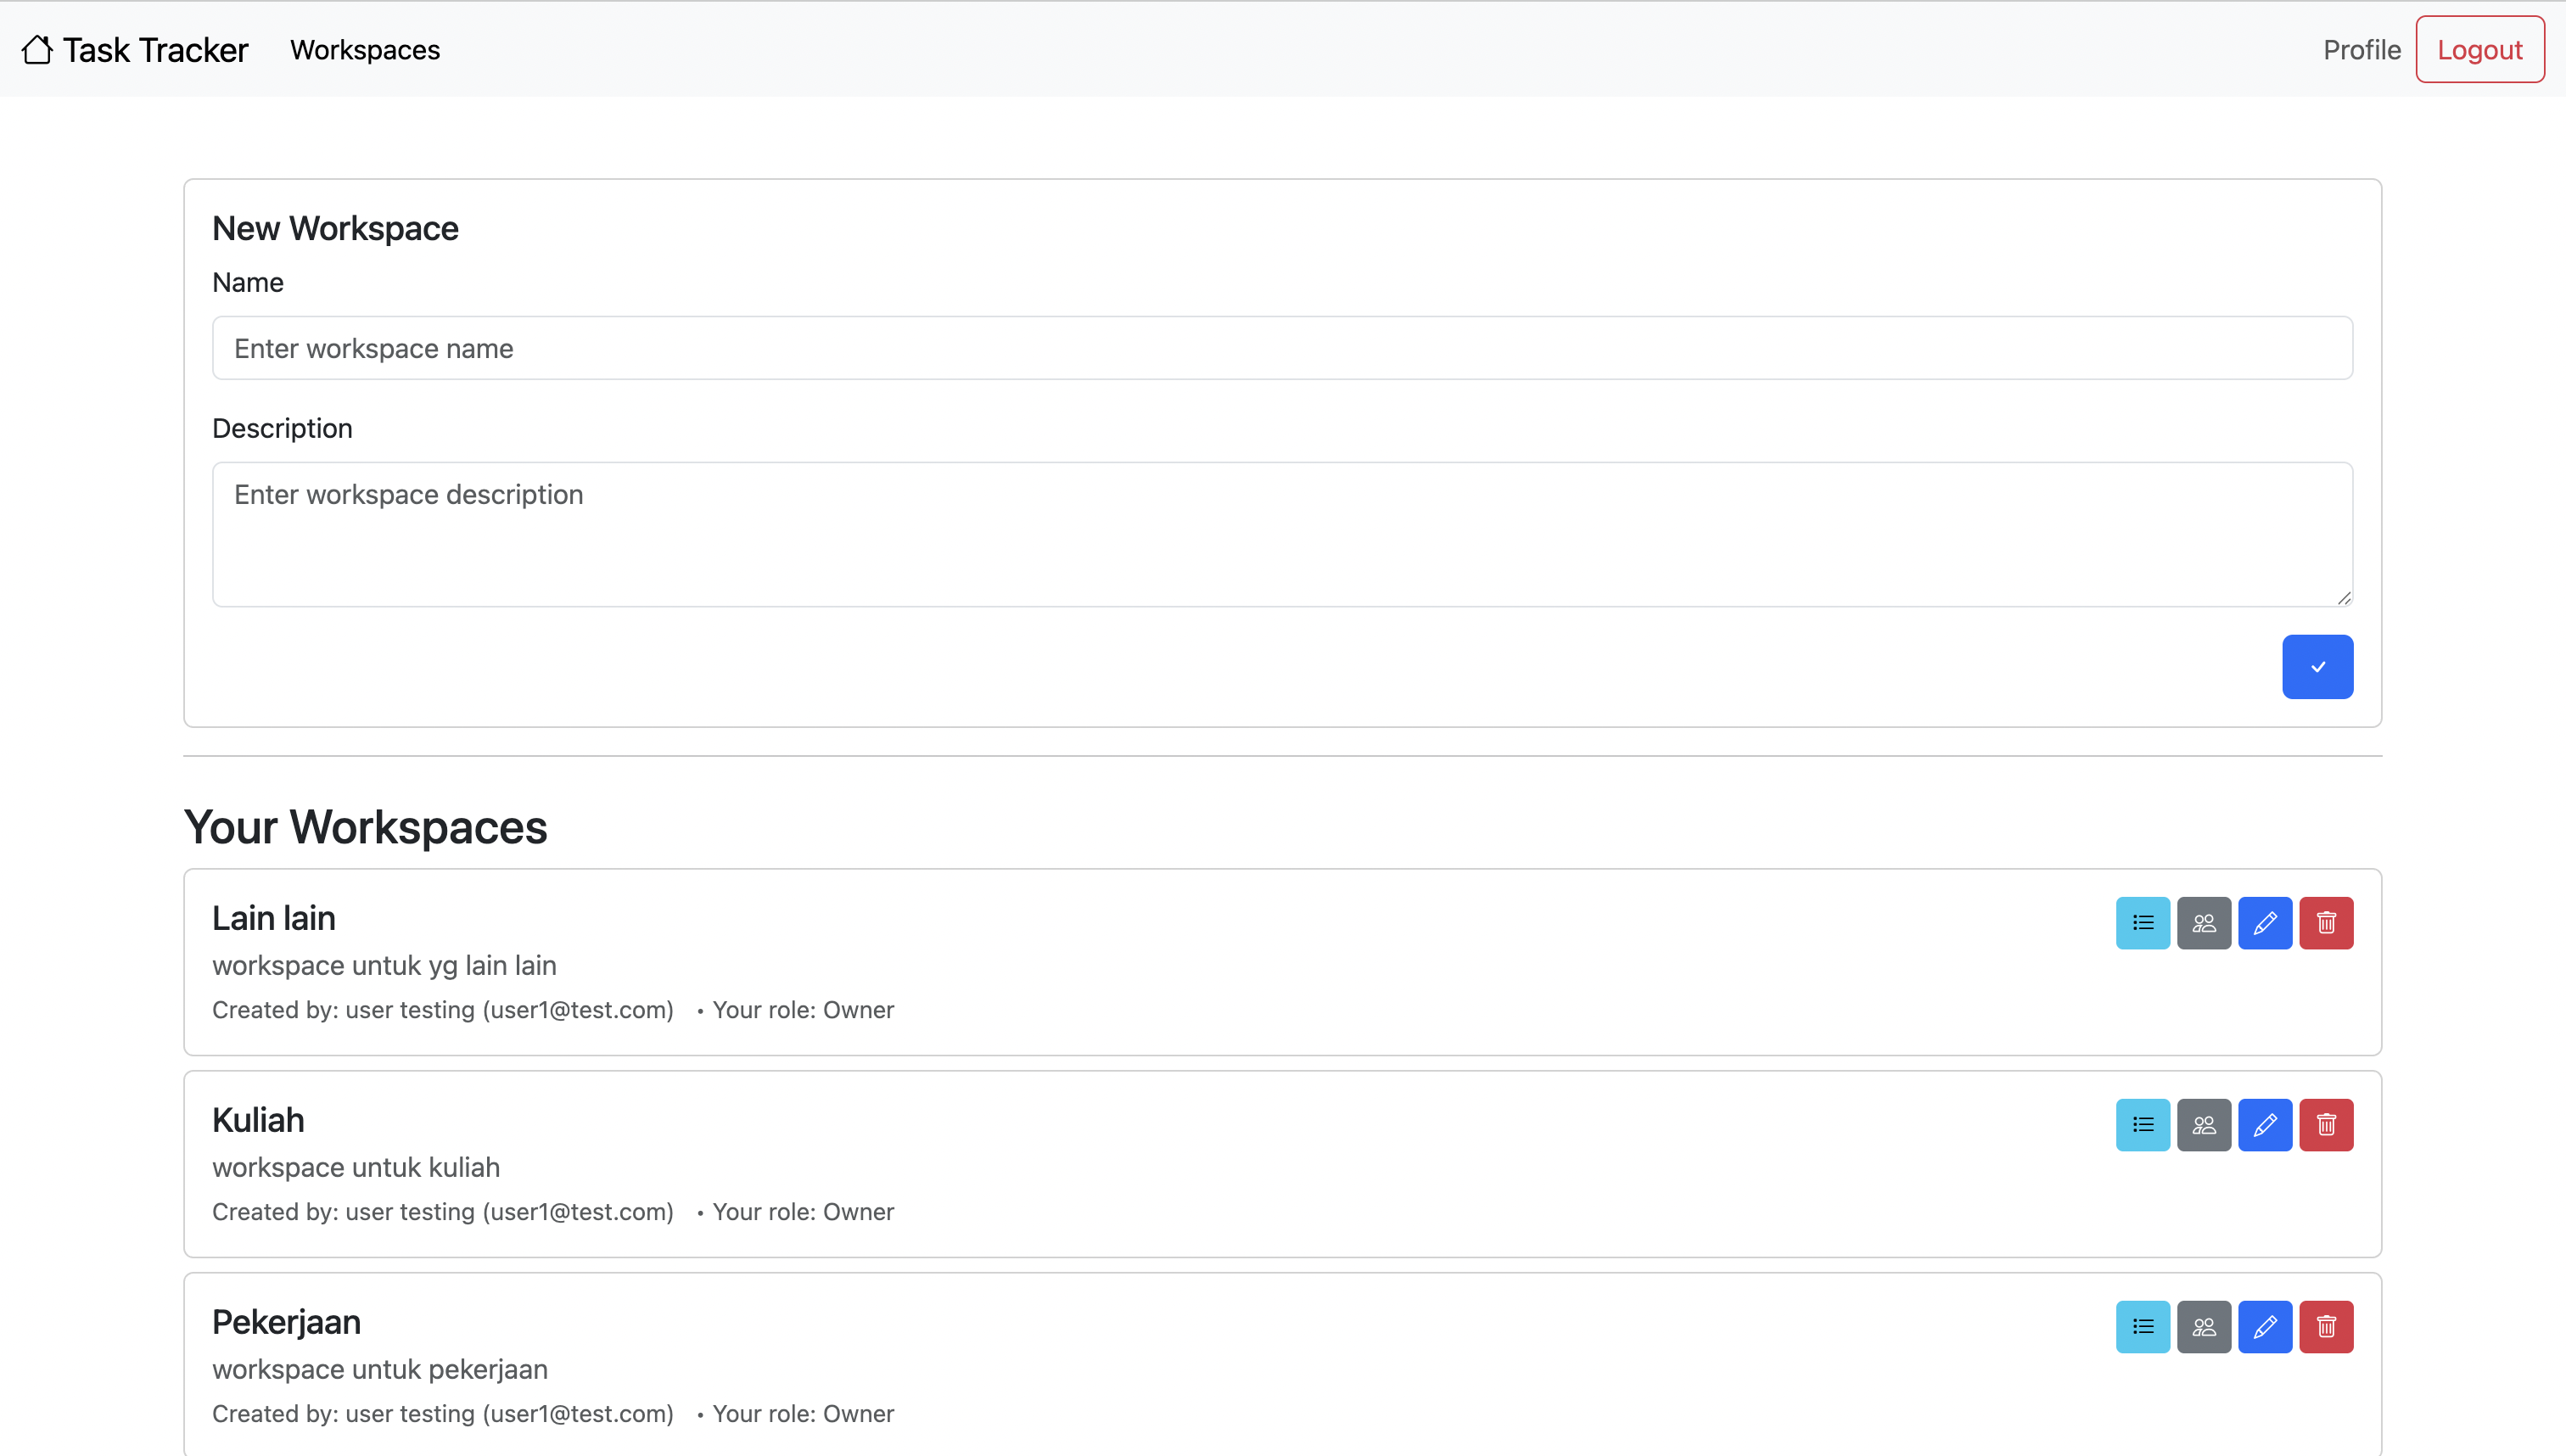
\includegraphics[width=1\textwidth]{assets/ui/list_workspace.png}
  \captionof{figure}{Tampilan UI List Workspace}
\end{center}
\begin{center}
  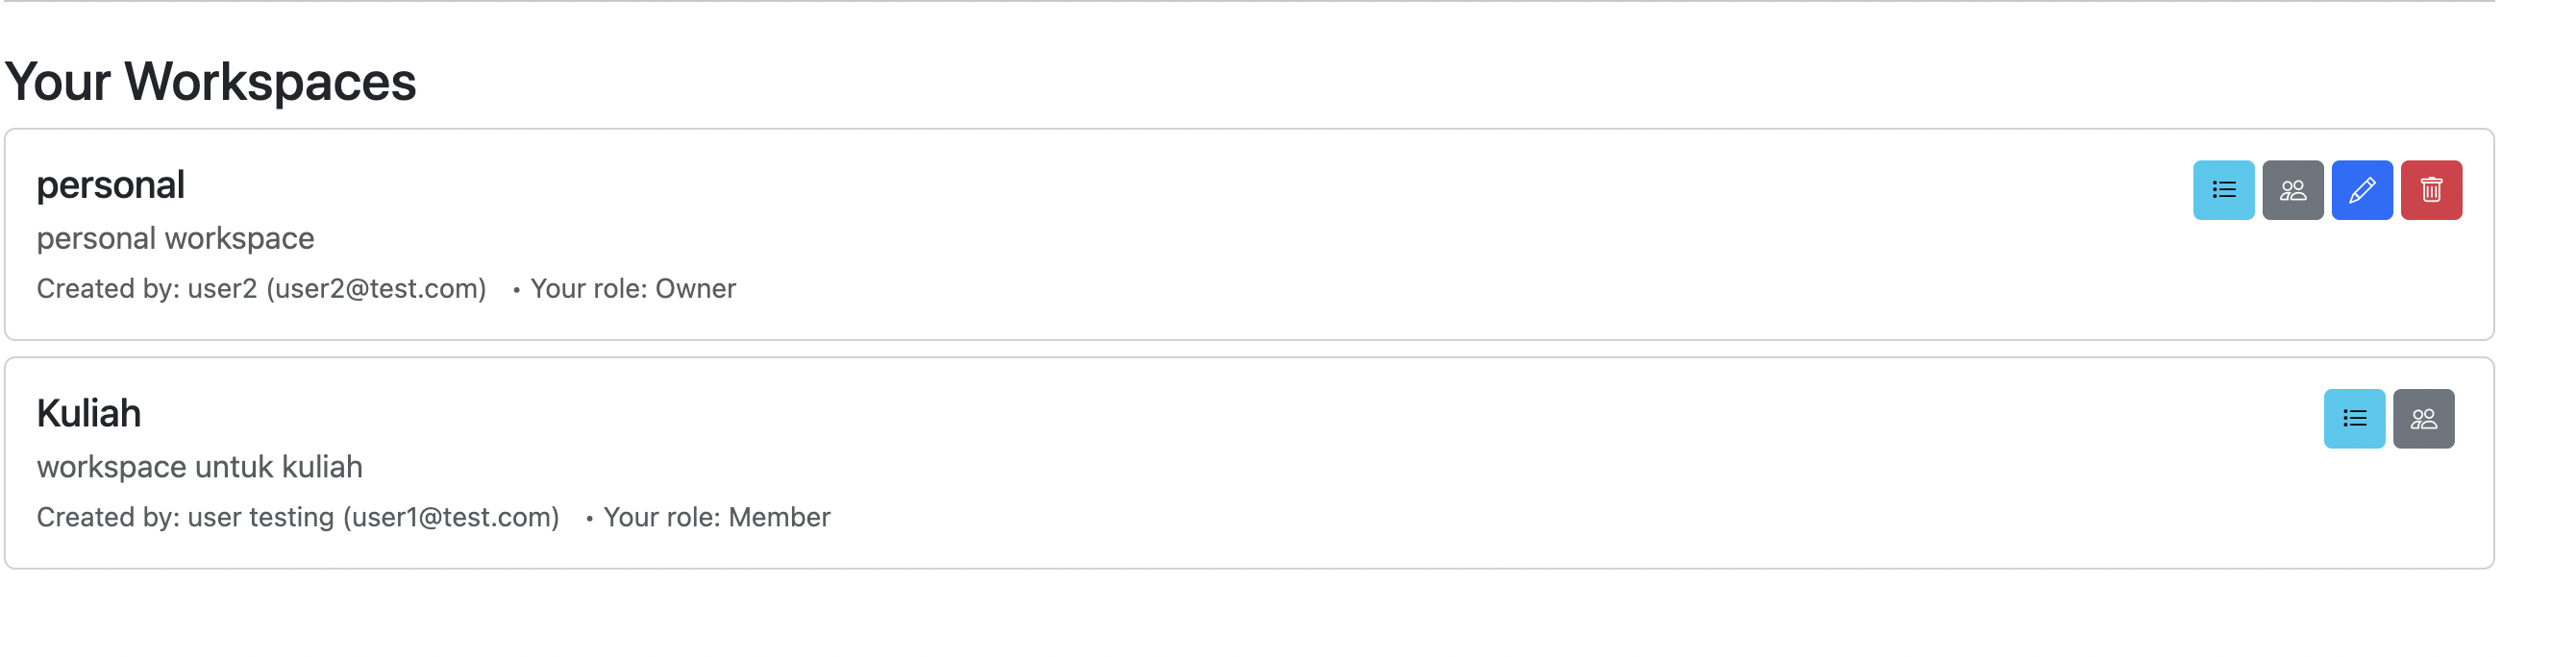
\includegraphics[width=1\textwidth]{assets/ui/workspace_list_row.png}
  \captionof{figure}{Detail UI Item List Workspace}
\end{center}

\subsection*{4.2.6 Tampilan UI Member}
halaman member digunakan untuk manajemen member pada workspace.
seperti menambahkan member baru, dan menghapus member / meninggalkan workspace.
halaman ini bisa diakses dengan cara mengklik icon member pada list workspace.
\begin{center}
  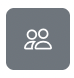
\includegraphics[width=0.1\textwidth]{assets/ui/workspace_member_icon.png}
  \captionof{figure}{Tampilan Icon Member}
\end{center}

setelah mengklik icon member, maka akan muncul tampilan seperti dibawah ini.
\begin{center}
  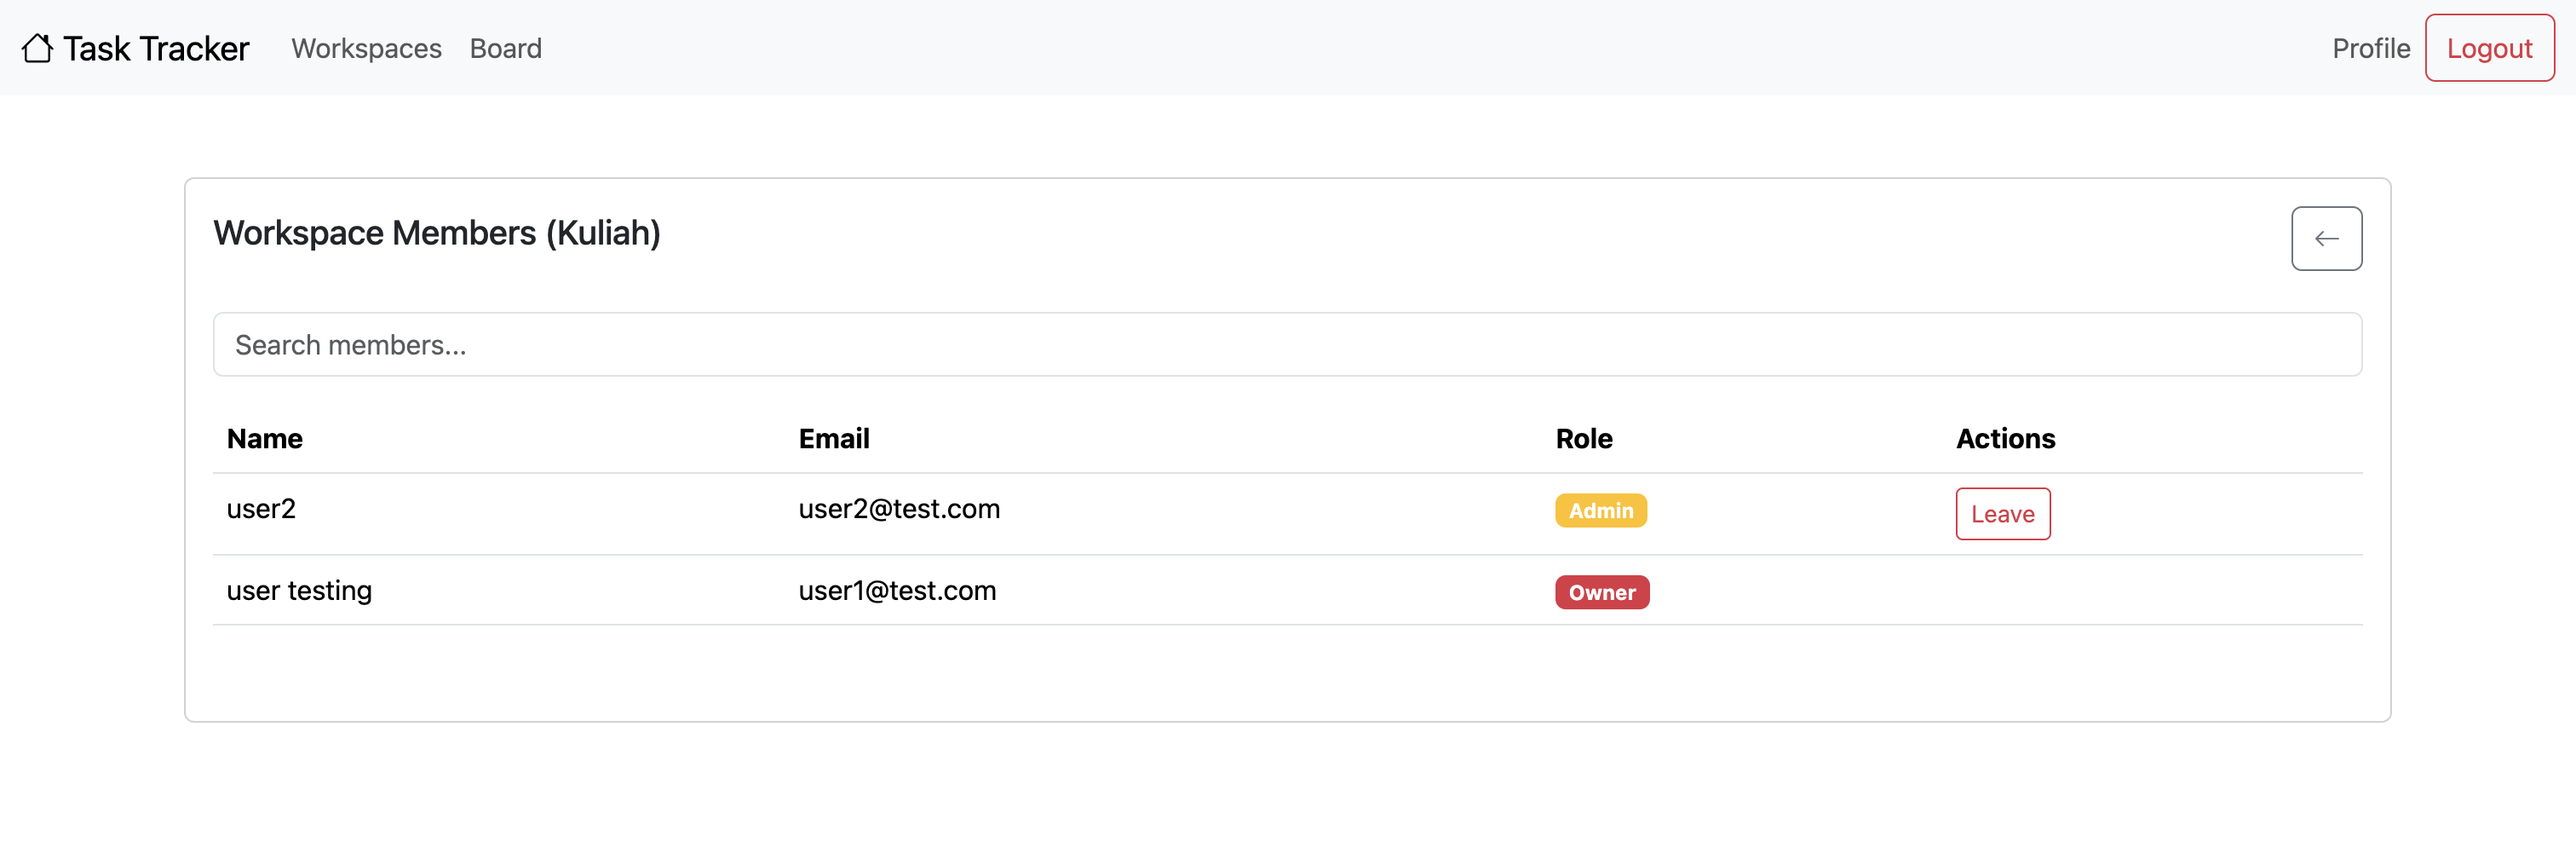
\includegraphics[width=1\textwidth]{assets/ui/list_member.png}
  \captionof{figure}{Tampilan UI List Member Biasa}
\end{center}
jika yang login bukan owner, akan ada tombol untuk meninggalkan workspace.
\begin{center}
  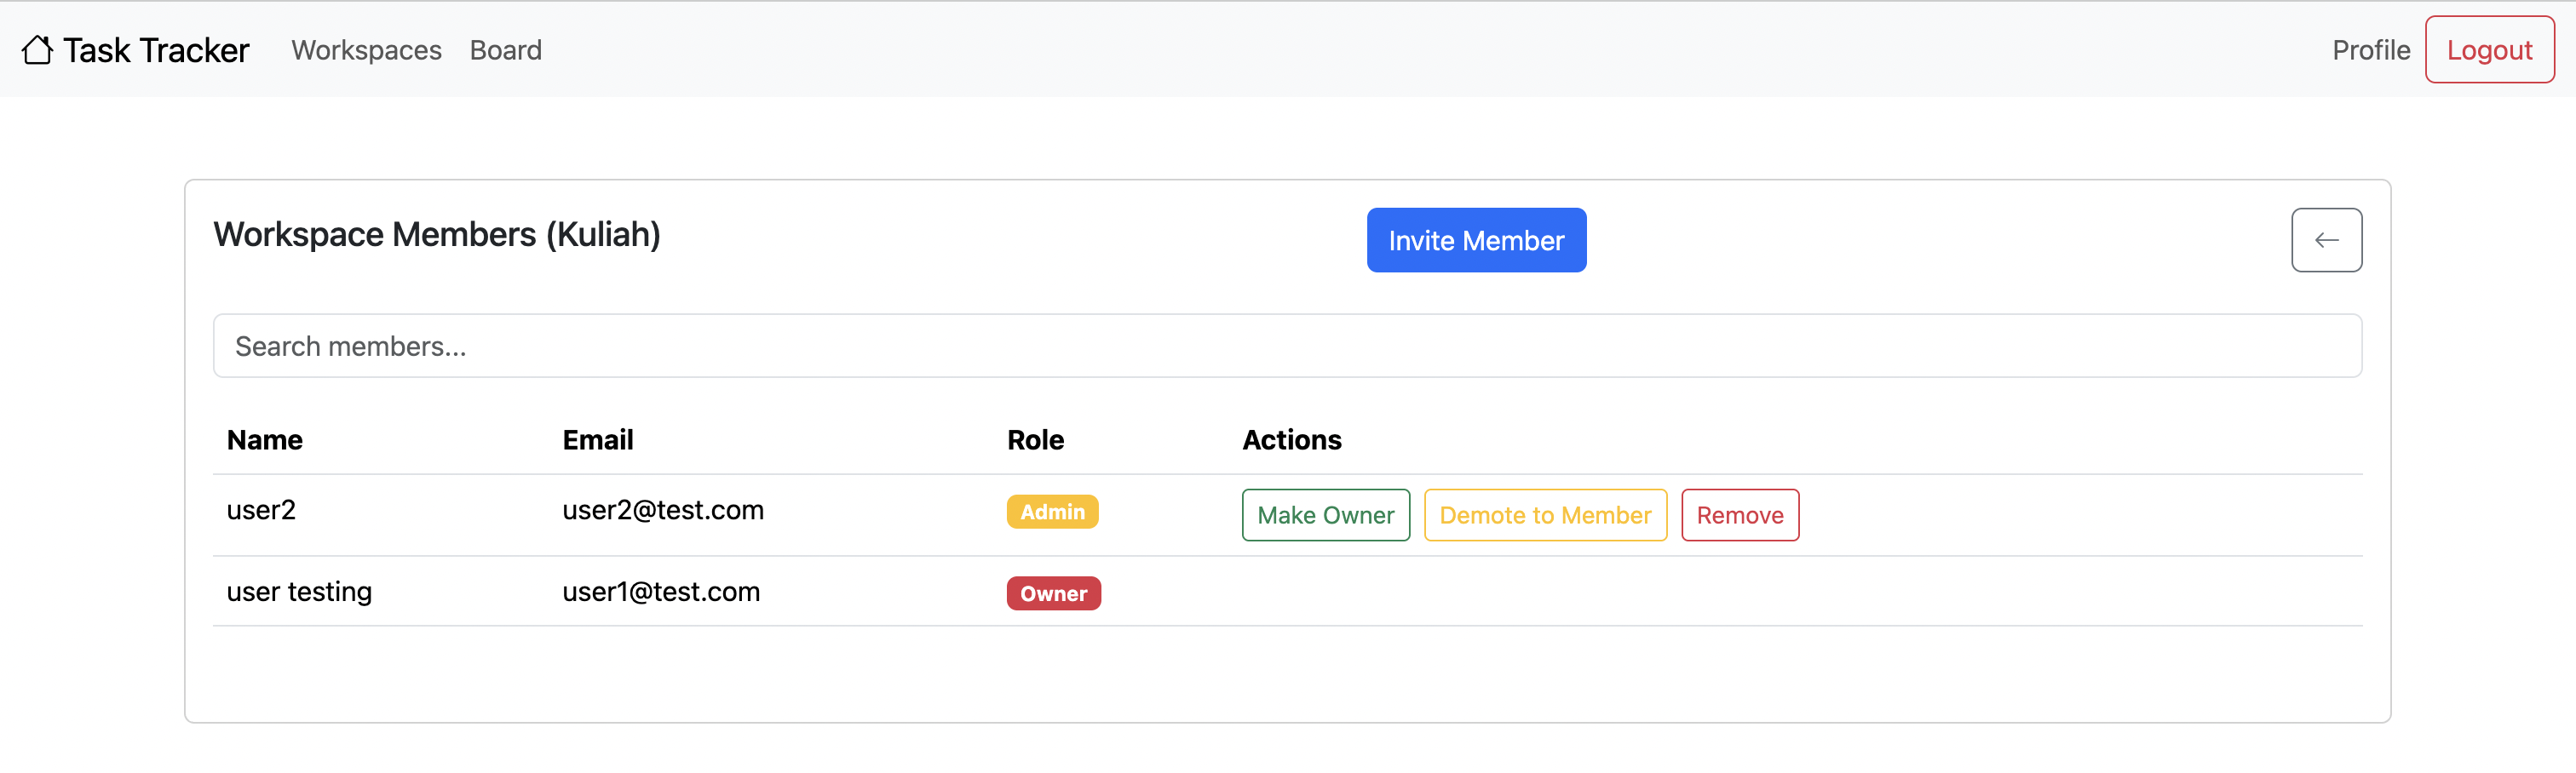
\includegraphics[width=1\textwidth]{assets/ui/list_member_owner.png}
  \captionof{figure}{Tampilan UI List Member Owner}
\end{center}
namun jika user yang login adalah owner, maka akan ada tombol untuk menghapus member lain.
di situ juga terdapat tombol untuk memasukan member baru ke dalam workspace.
\begin{center}
  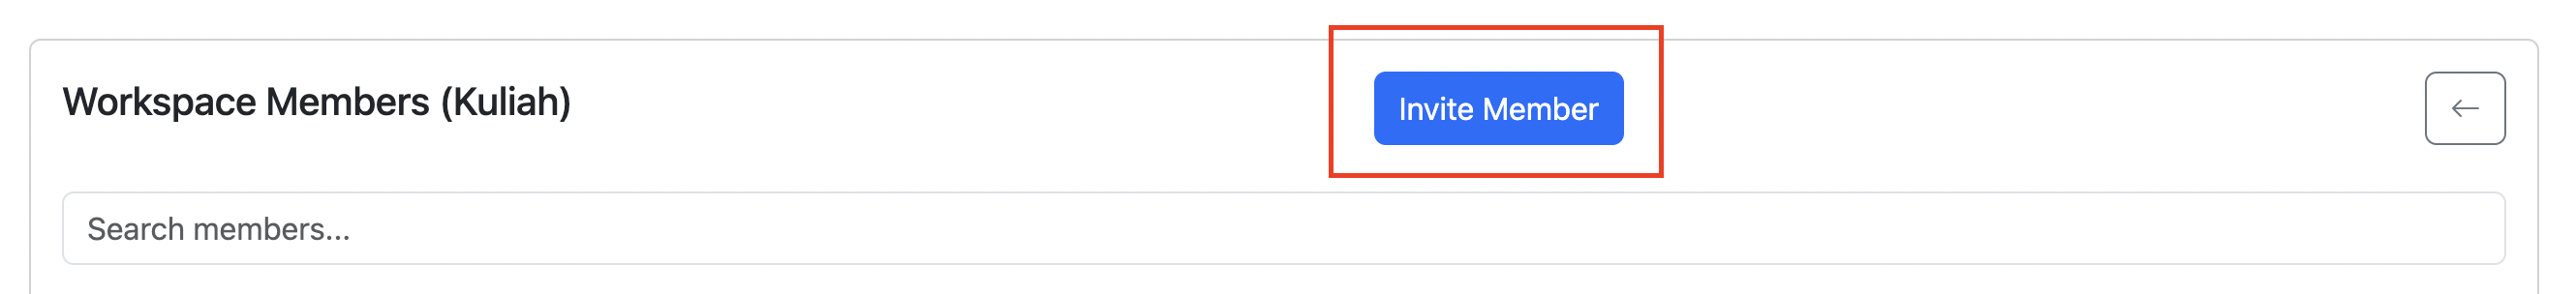
\includegraphics[width=1\textwidth]{assets/ui/invite_member_button_location.png}
  \captionof{figure}{Tampilan Detail Lokasi Tombol Invite Member}
\end{center}
setelah mengklik tombol invite member, maka akan muncul form untuk memasukan email member yang akan diundang.
\begin{center}
  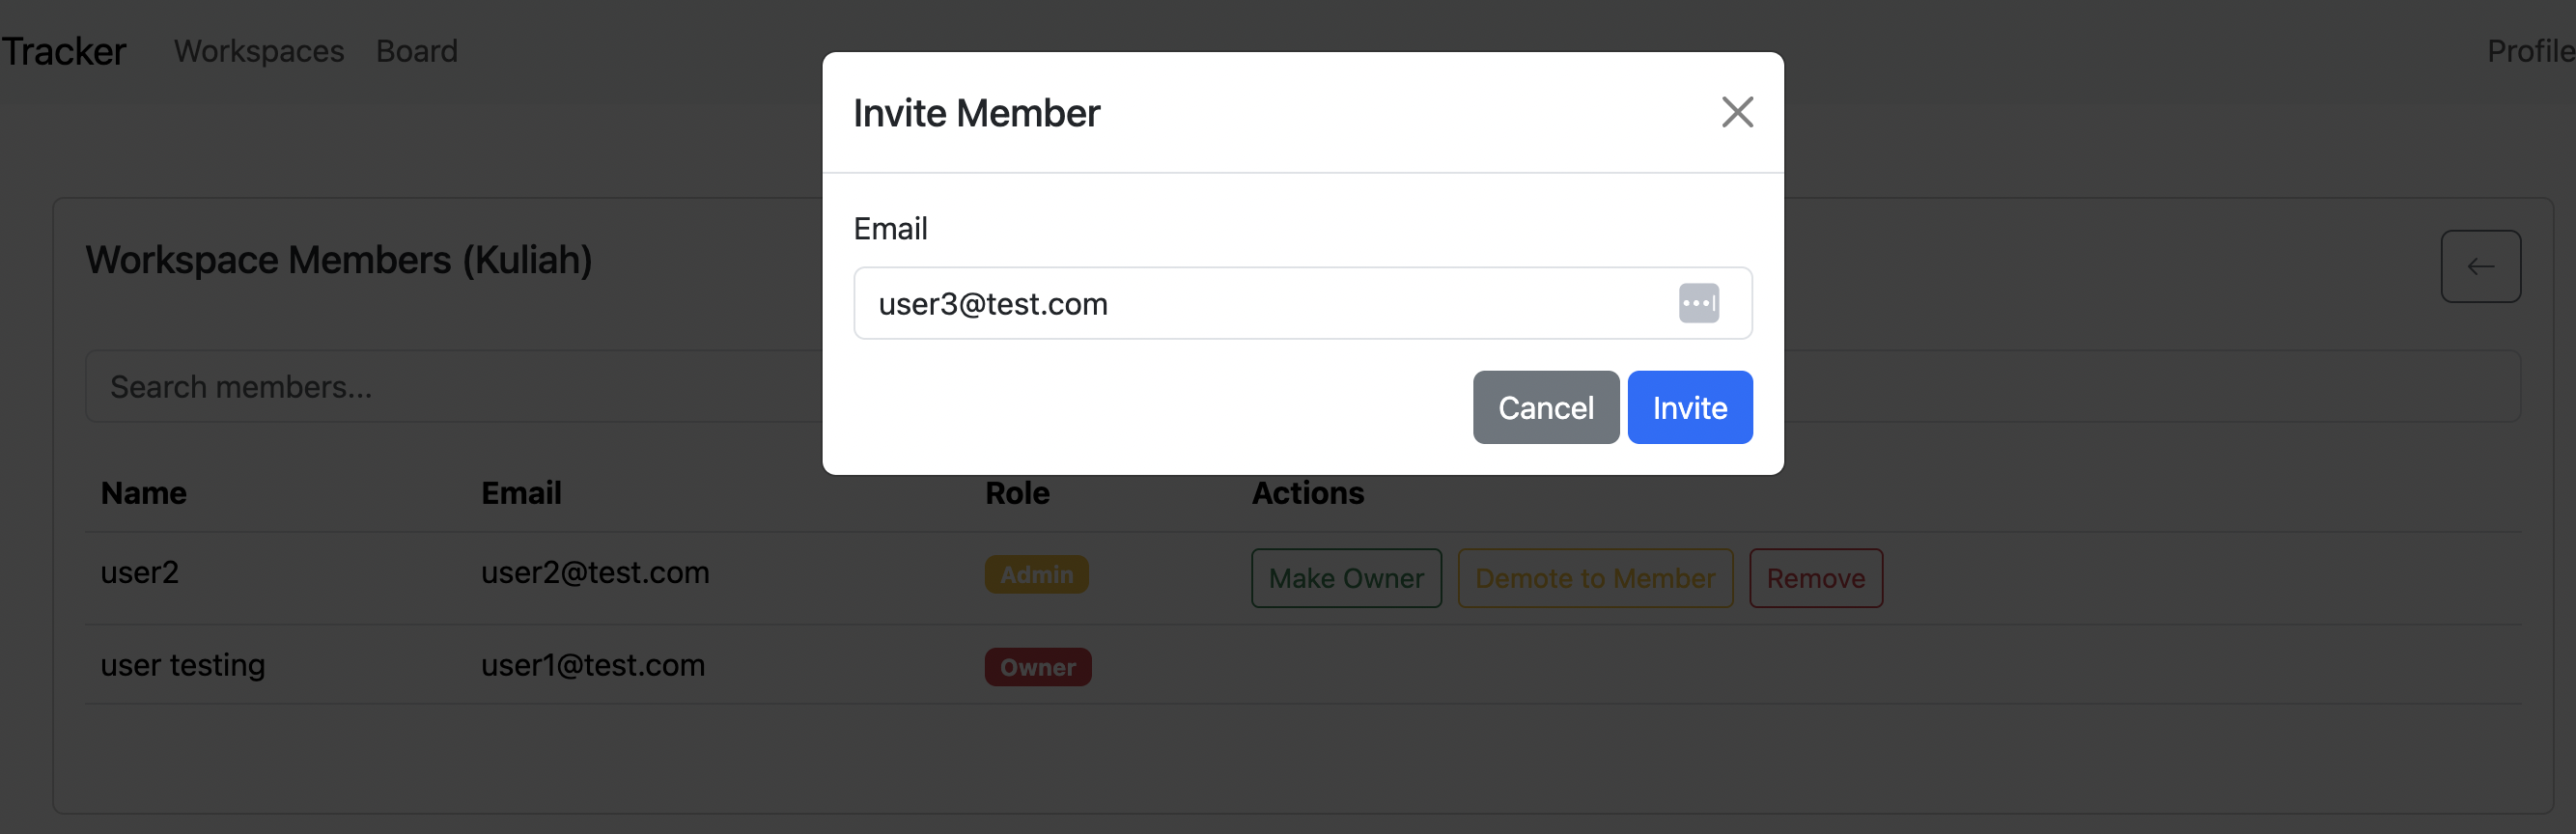
\includegraphics[width=1\textwidth]{assets/ui/invite_member_form_filled.png}
  \captionof{figure}{Tampilan UI Form Invite Member}
\end{center}
setelah mengisi email member yang akan diundang, dan mengklik tombol invite, maka member yang diundang akan masuk kedalam list member.
\begin{center}
  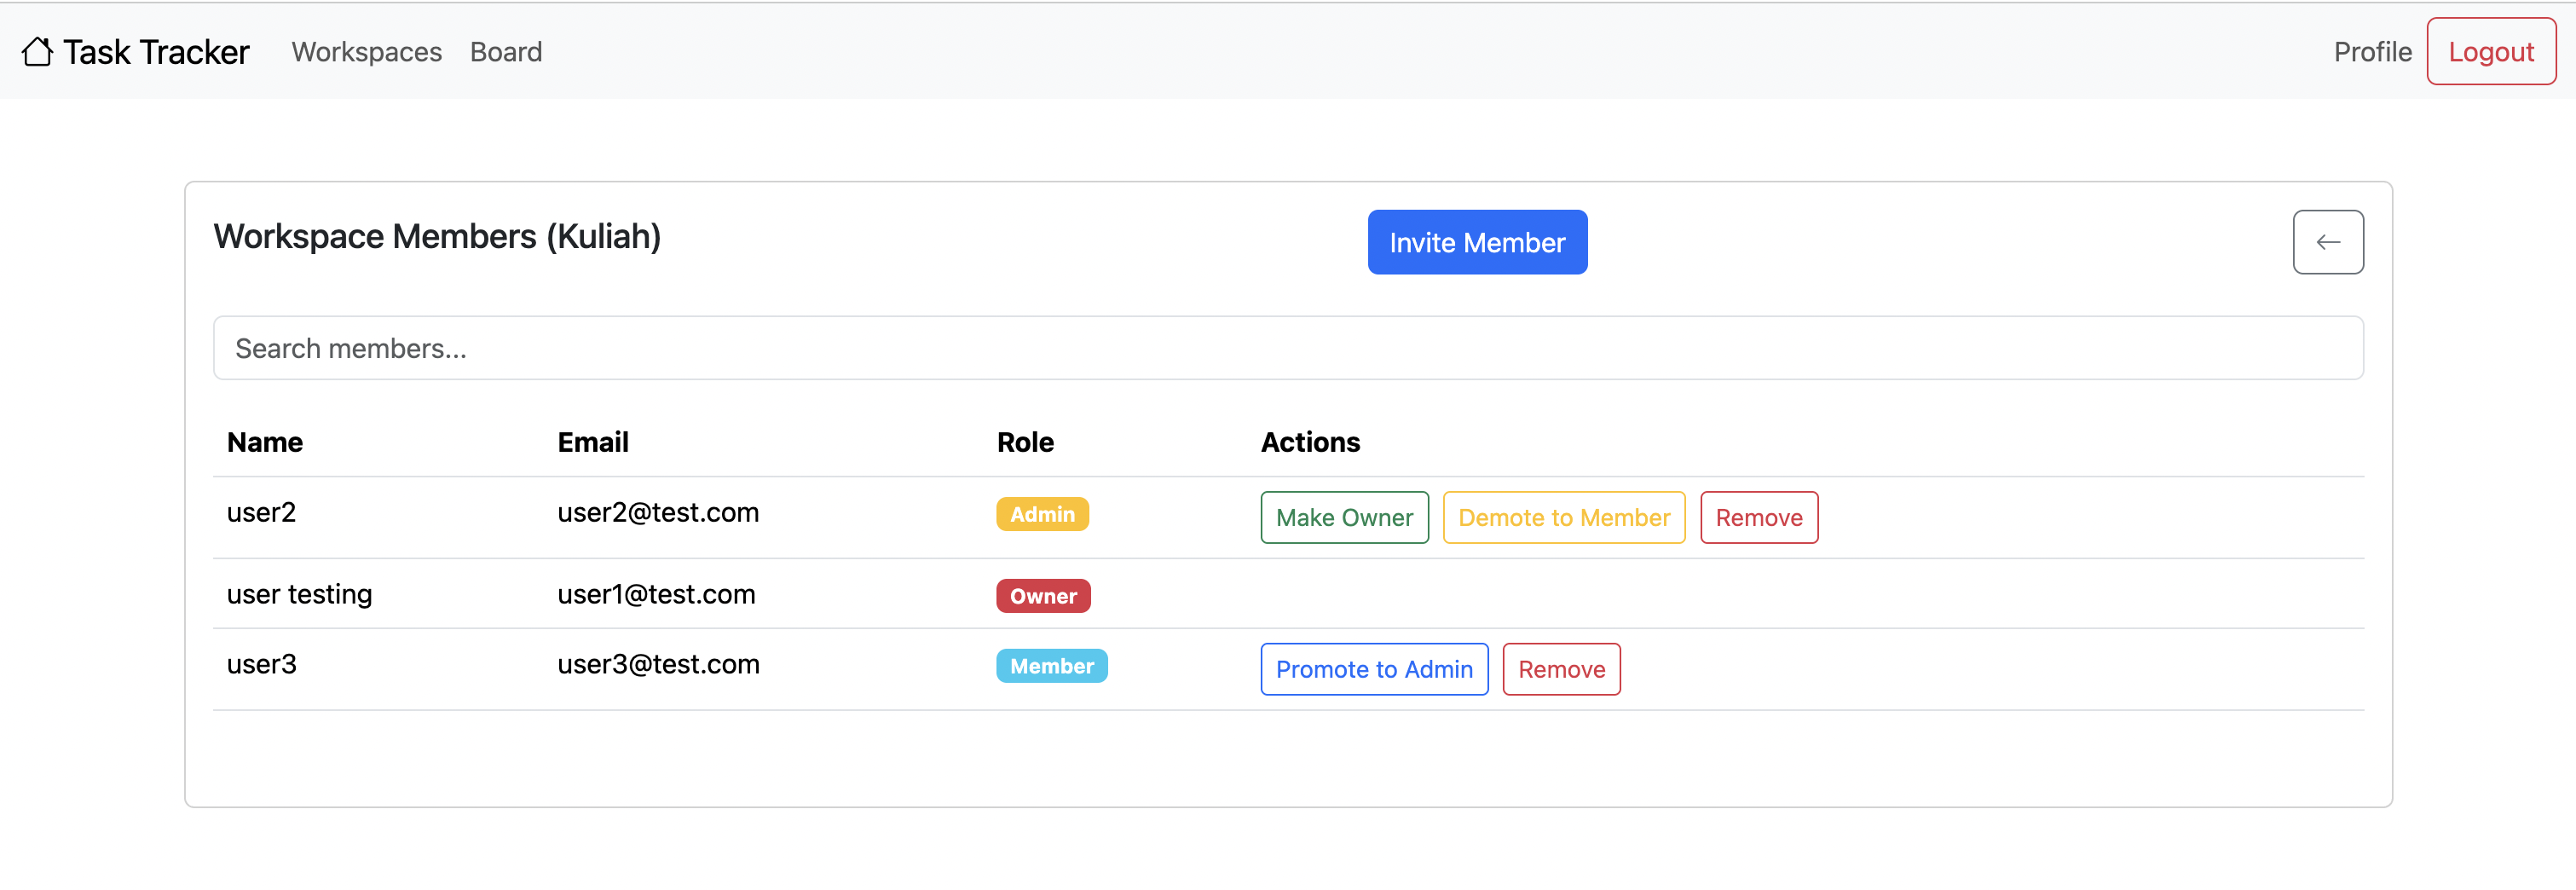
\includegraphics[width=1\textwidth]{assets/ui/list_member_complete_role.png}
  \captionof{figure}{Tampilan UI List Member Setelah Invite Member}
\end{center}
di bagian kolom actions, juga terdapat beberapa tombol yang bisa digunakan.
\begin{center}
  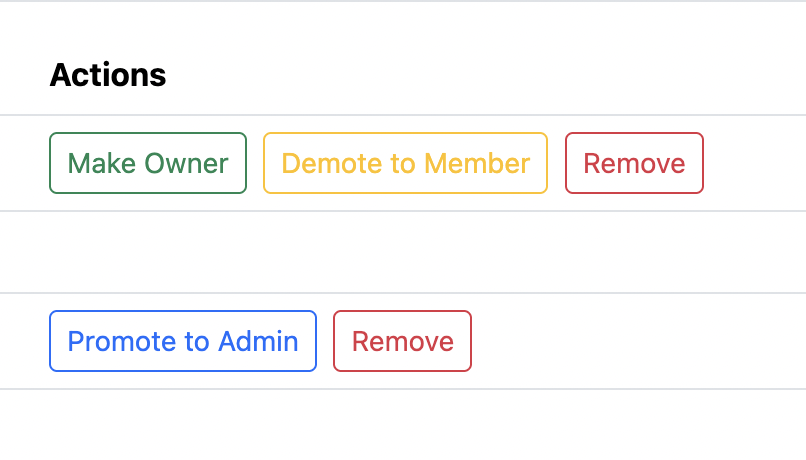
\includegraphics[width=1\textwidth]{assets/ui/list_member_actions.png}
  \captionof{figure}{Tampilan Detail Lokasi Tombol Actions}
\end{center}
\begin{itemize}
  \item tombol "Make Owner" digunakan untuk mengubah member menjadi owner.
  \item tombol "Remove" digunakan untuk menghapus member dari workspace.
  \item tombol "Demote Member" digunakan untuk menurunkan role member menjadi member biasa.
  \item tombol "Promote Admin" digunakan untuk menaikkan role member menjadi admin.
\end{itemize}

\subsection*{4.2.7 Tampilan UI Task Board}
halaman ini digunakan untuk menampilkan task yang ada di dalam workspace dengan status todo, in progress, dan done.
dafta task dengan status tersebut akan di tampilkan di dalam board yang terdiri dari 3 kolom, yaitu todo, in progress, dan done.
\begin{center}
  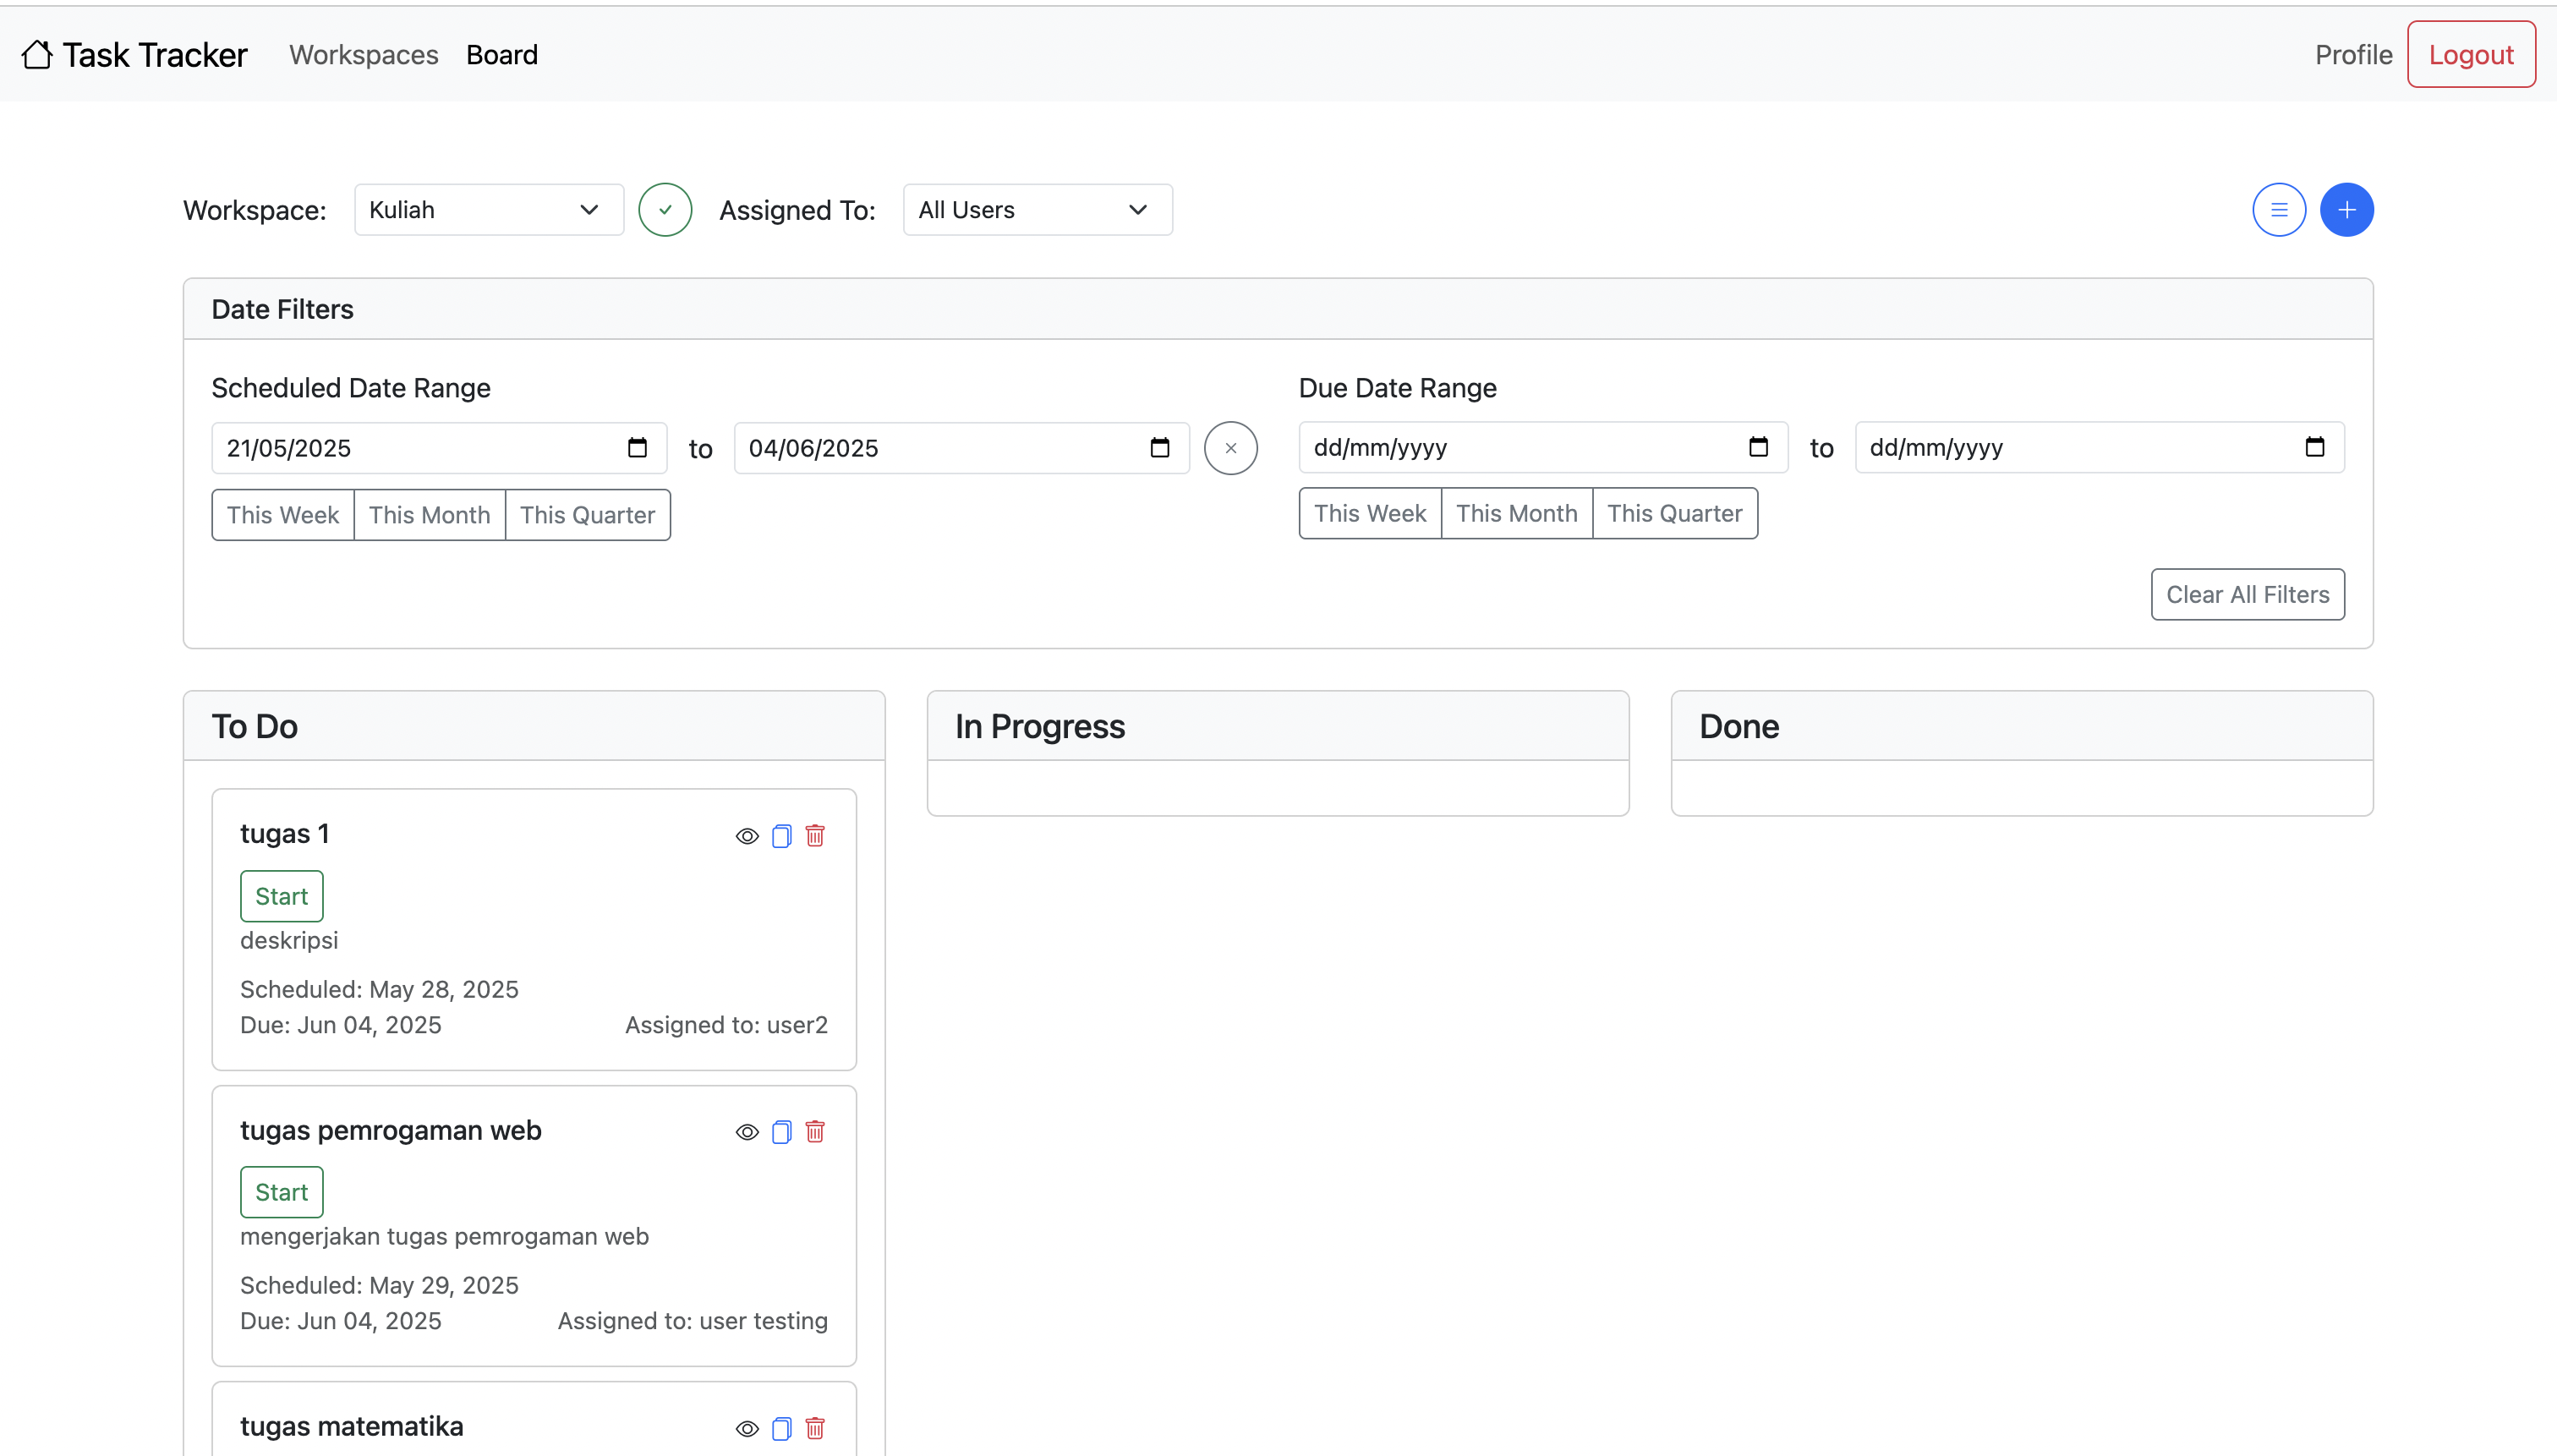
\includegraphics[width=1\textwidth]{assets/ui/task_board.png}
  \captionof{figure}{Tampilan UI Task Board}
\end{center}
di halaman ini juga terdapat beberapa filter yang bisa digunakan untuk memfilter task yang ada di dalam board.
user juga bisa memilih workspace yang akan digunakan untuk menampilkan task.
\\ untuk membuat task baru, user bisa mengklik tombol "+" yang terdapat di pojok kanan atas board.
setelah diklik, maka akan muncul form untuk membuat task baru.
\begin{center}
  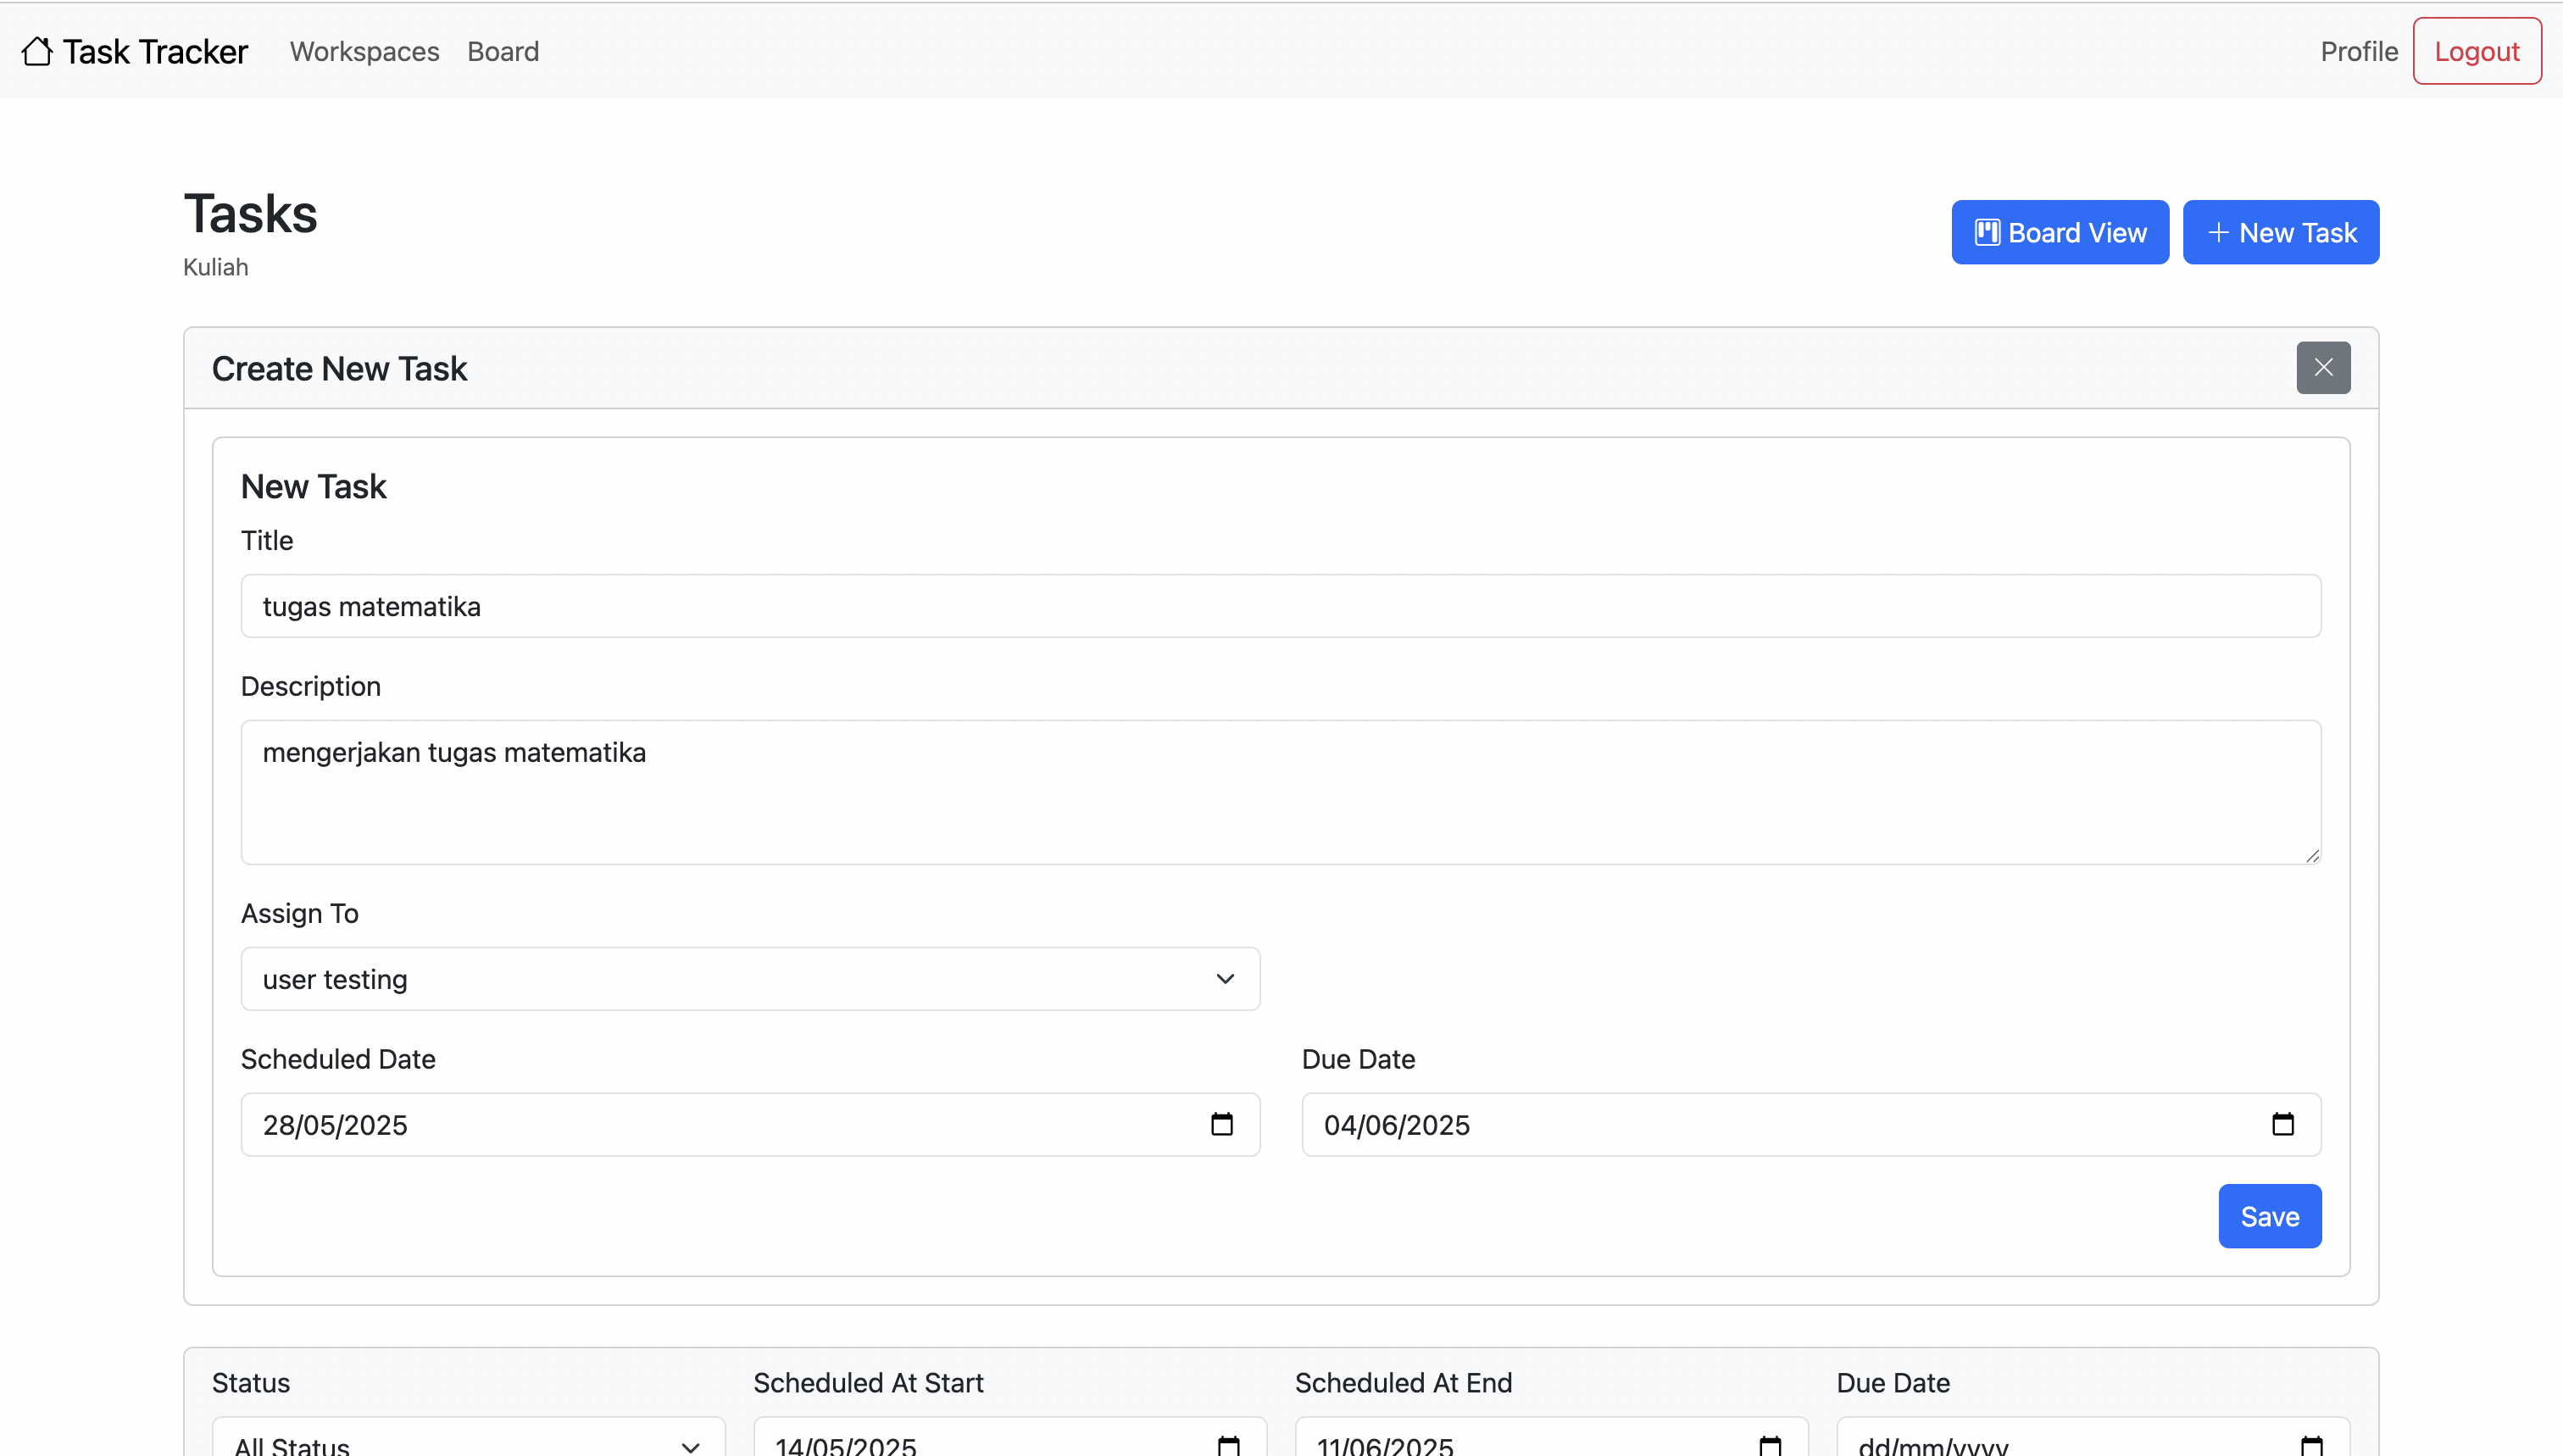
\includegraphics[width=1\textwidth]{assets/ui/task_create_filled.png}
  \captionof{figure}{Tampilan UI Form Create Task}
\end{center}
setelah mengisi form, dan mengklik tombol "Save", maka task baru akan muncul di dalam board di status todo.
\\ berikut adalah tampilan detail ui item task.
\begin{center}
  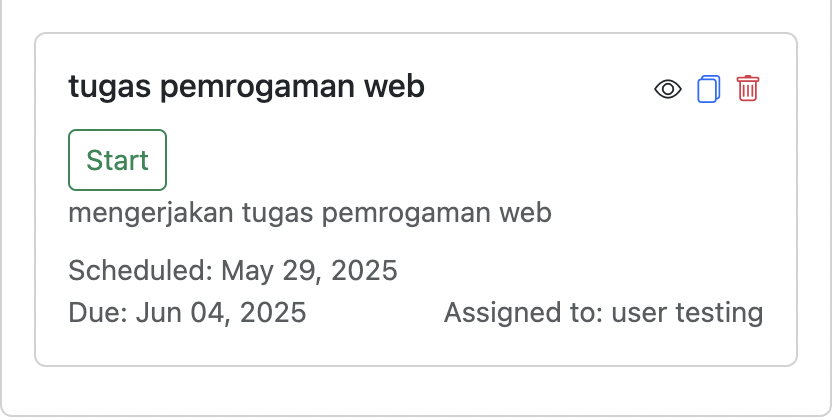
\includegraphics[width=1\textwidth]{assets/ui/task_board_item.png}
  \captionof{figure}{Tampilan UI Item Task}
\end{center}
disitu terdapat beberapa tombol yang bisa digunakan.
\\ di pojok atas kanan, terdapat tombol dengan beberapa icon.
\begin{center}
  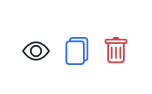
\includegraphics[width=0.3\textwidth]{assets/ui/task_board_item_actions.png}
  \captionof{figure}{Tampilan Detail Lokasi Tombol Actions}
\end{center}
dari sebelah kiri ke ke kanan
\begin{itemize}
  \item tombol dengan icon "mata" digunakan untuk melihat detail task dalam bentuk form yang bisa di edit.
  \item tombol "persegi saling bertumpuk" digunakan untuk duplikasi task.
  \item tombol "kotak sampah" digunakan untuk menghapus task.
\end{itemize}
saat klik tombol "mata", maka akan muncul detail task yang ada di dalam task tersebut.
\begin{center}
  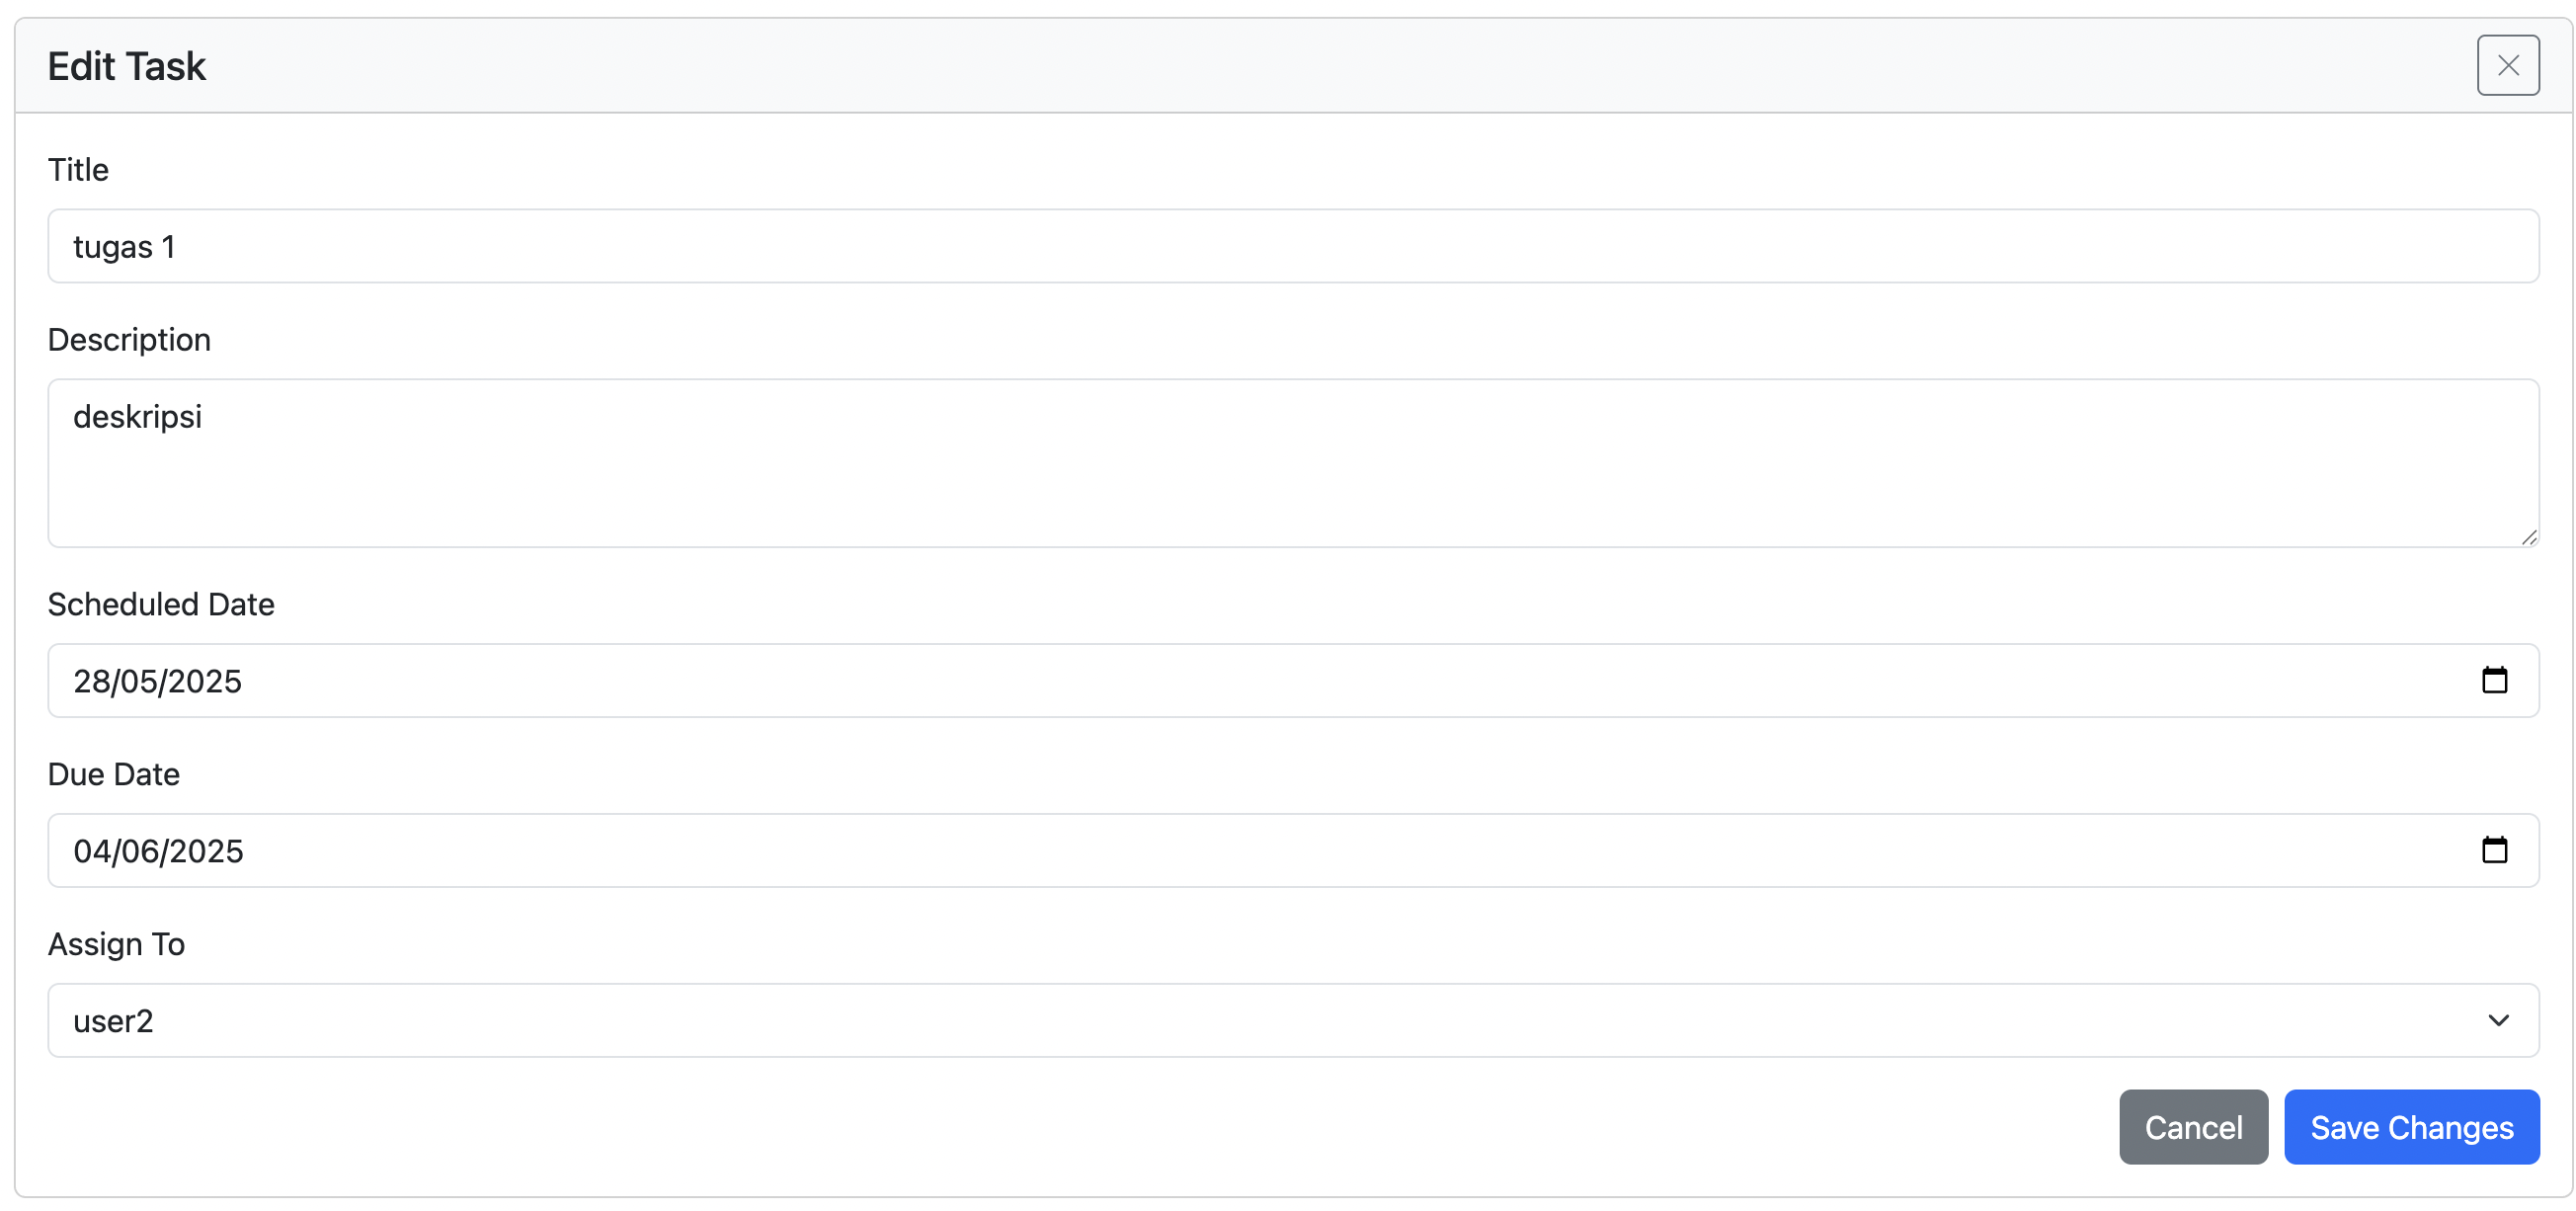
\includegraphics[width=1\textwidth]{assets/ui/board_task_edit.png}
  \captionof{figure}{Tampilan Detail Item Task dengan Form Edit}
\end{center}
saat klik tombol "persegi saling bertumpuk", maka akan muncul form untuk membuat task baru dengan data yang sama dengan task yang dipilih.
\begin{center}
  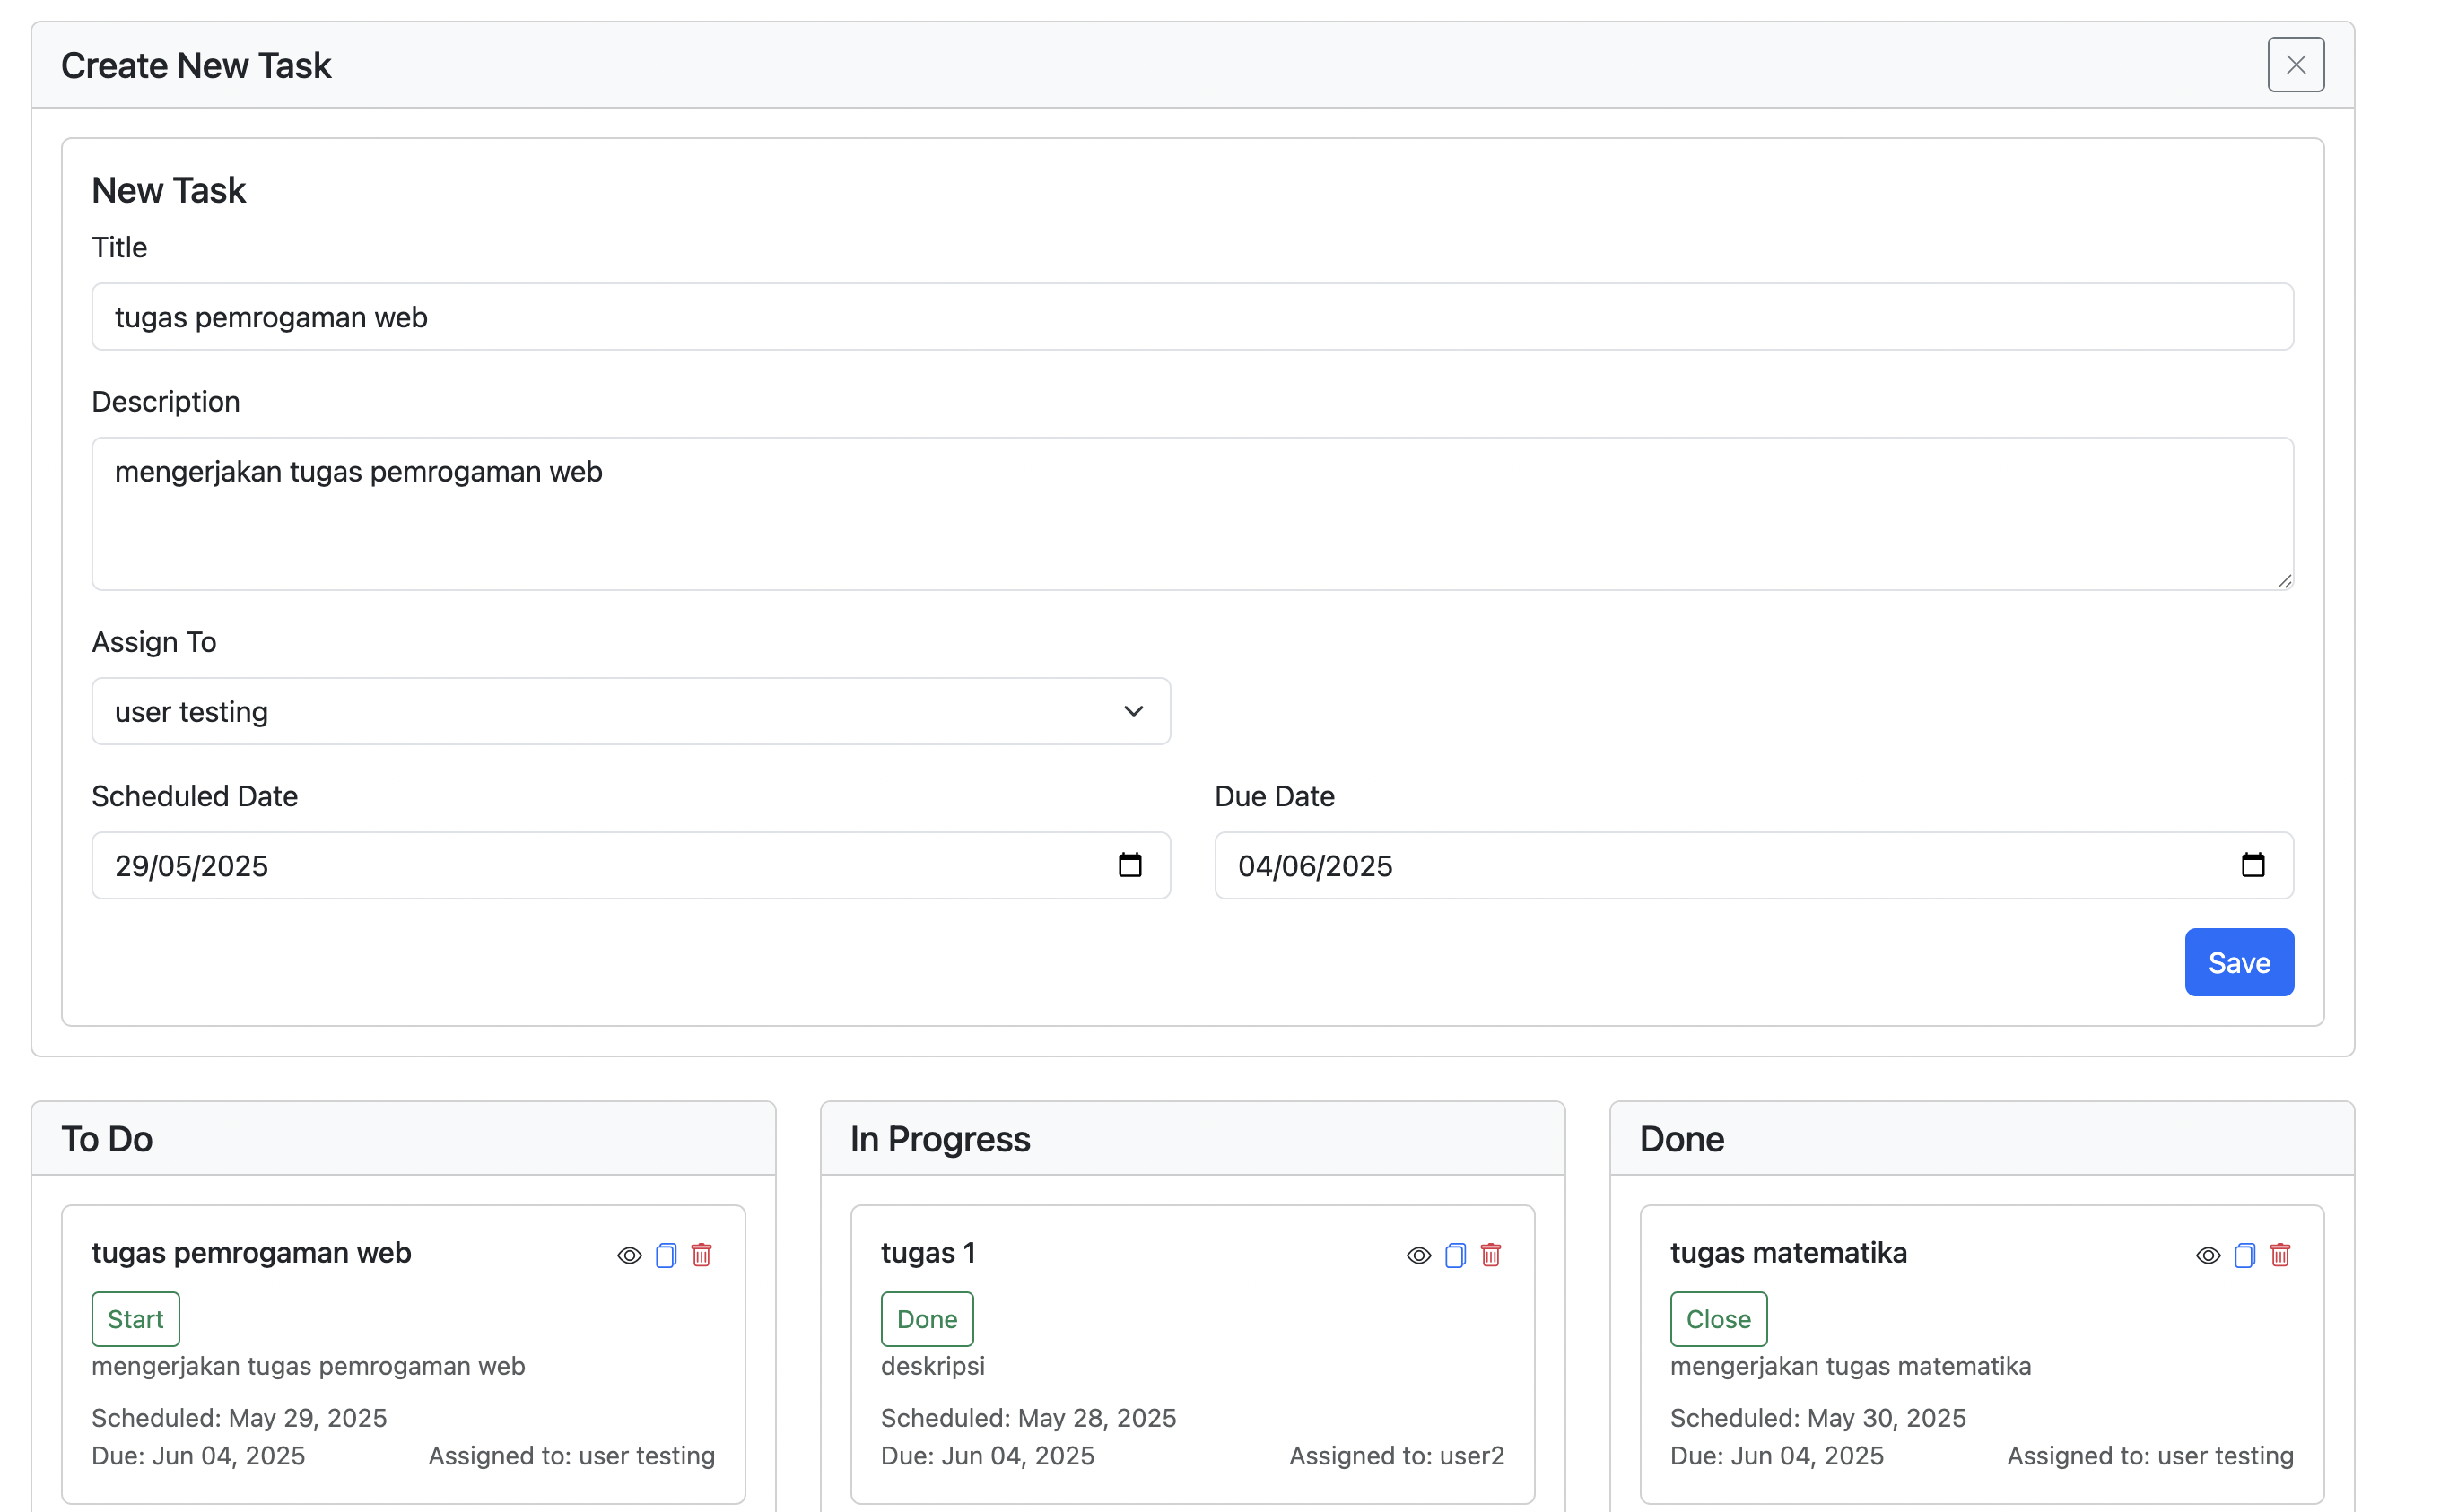
\includegraphics[width=1\textwidth]{assets/ui/duplicate_task_form.png}
  \captionof{figure}{Tampilan UI Form Duplicate Task}
\end{center}
di antara judul dan deskripsi task juga terdapat tombol bertulis "Start". \
tombol ini digunakan untuk memindahkan status task ke status selanjutnya.
selain "Start", juga terdapat tombol "Done" dan "Close".
\begin{center}
  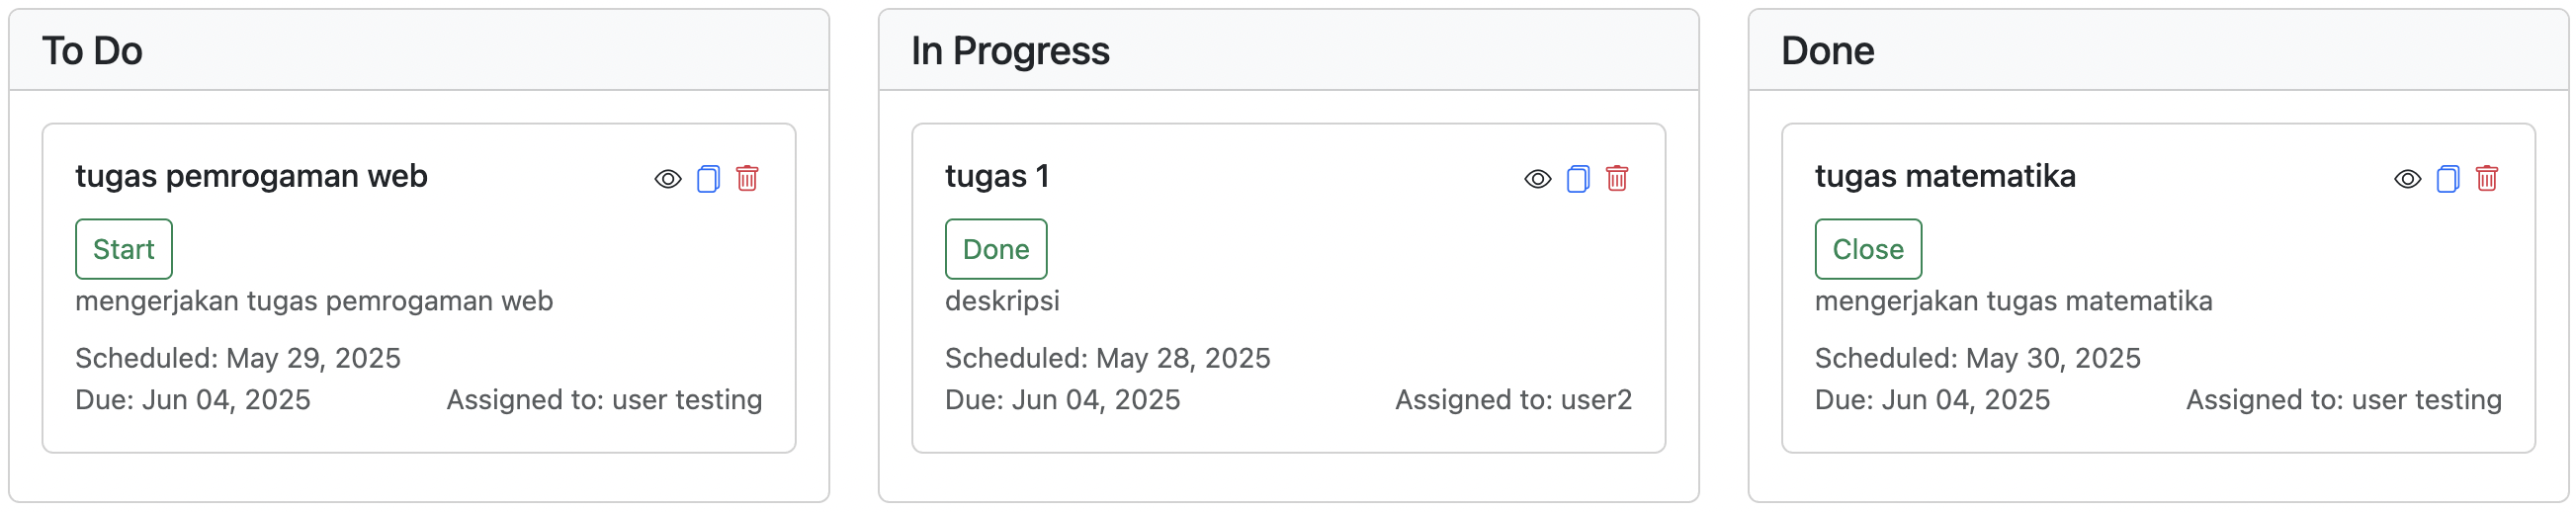
\includegraphics[width=1\textwidth]{assets/ui/task_board_item_complete_status.png}
  \captionof{figure}{Tampilan Detail Item Task dengan berbagai Tombol Ubah Status}
\end{center}
di sebelah kanan atas board, selain ada tombol untuk membuat task baru, juga terdapat tombol untuk masuk ke halaman list task.
\begin{center}
  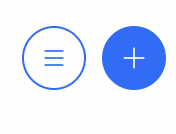
\includegraphics[width=0.3\textwidth]{assets/ui/board_top_right_buttons.png}
  \captionof{figure}{Tampilan Detail Lokasi Tombol Pojok Kanan Atas Task Board}
\end{center}
kalian bisa mengklik tombol 3 garis horizontal yang saling sejajar.
itu akan mengarahkan kalian ke halaman list task. di halaman ini, kalian bisa melihat semua task yang ada di dalam workspace.
\begin{center}
  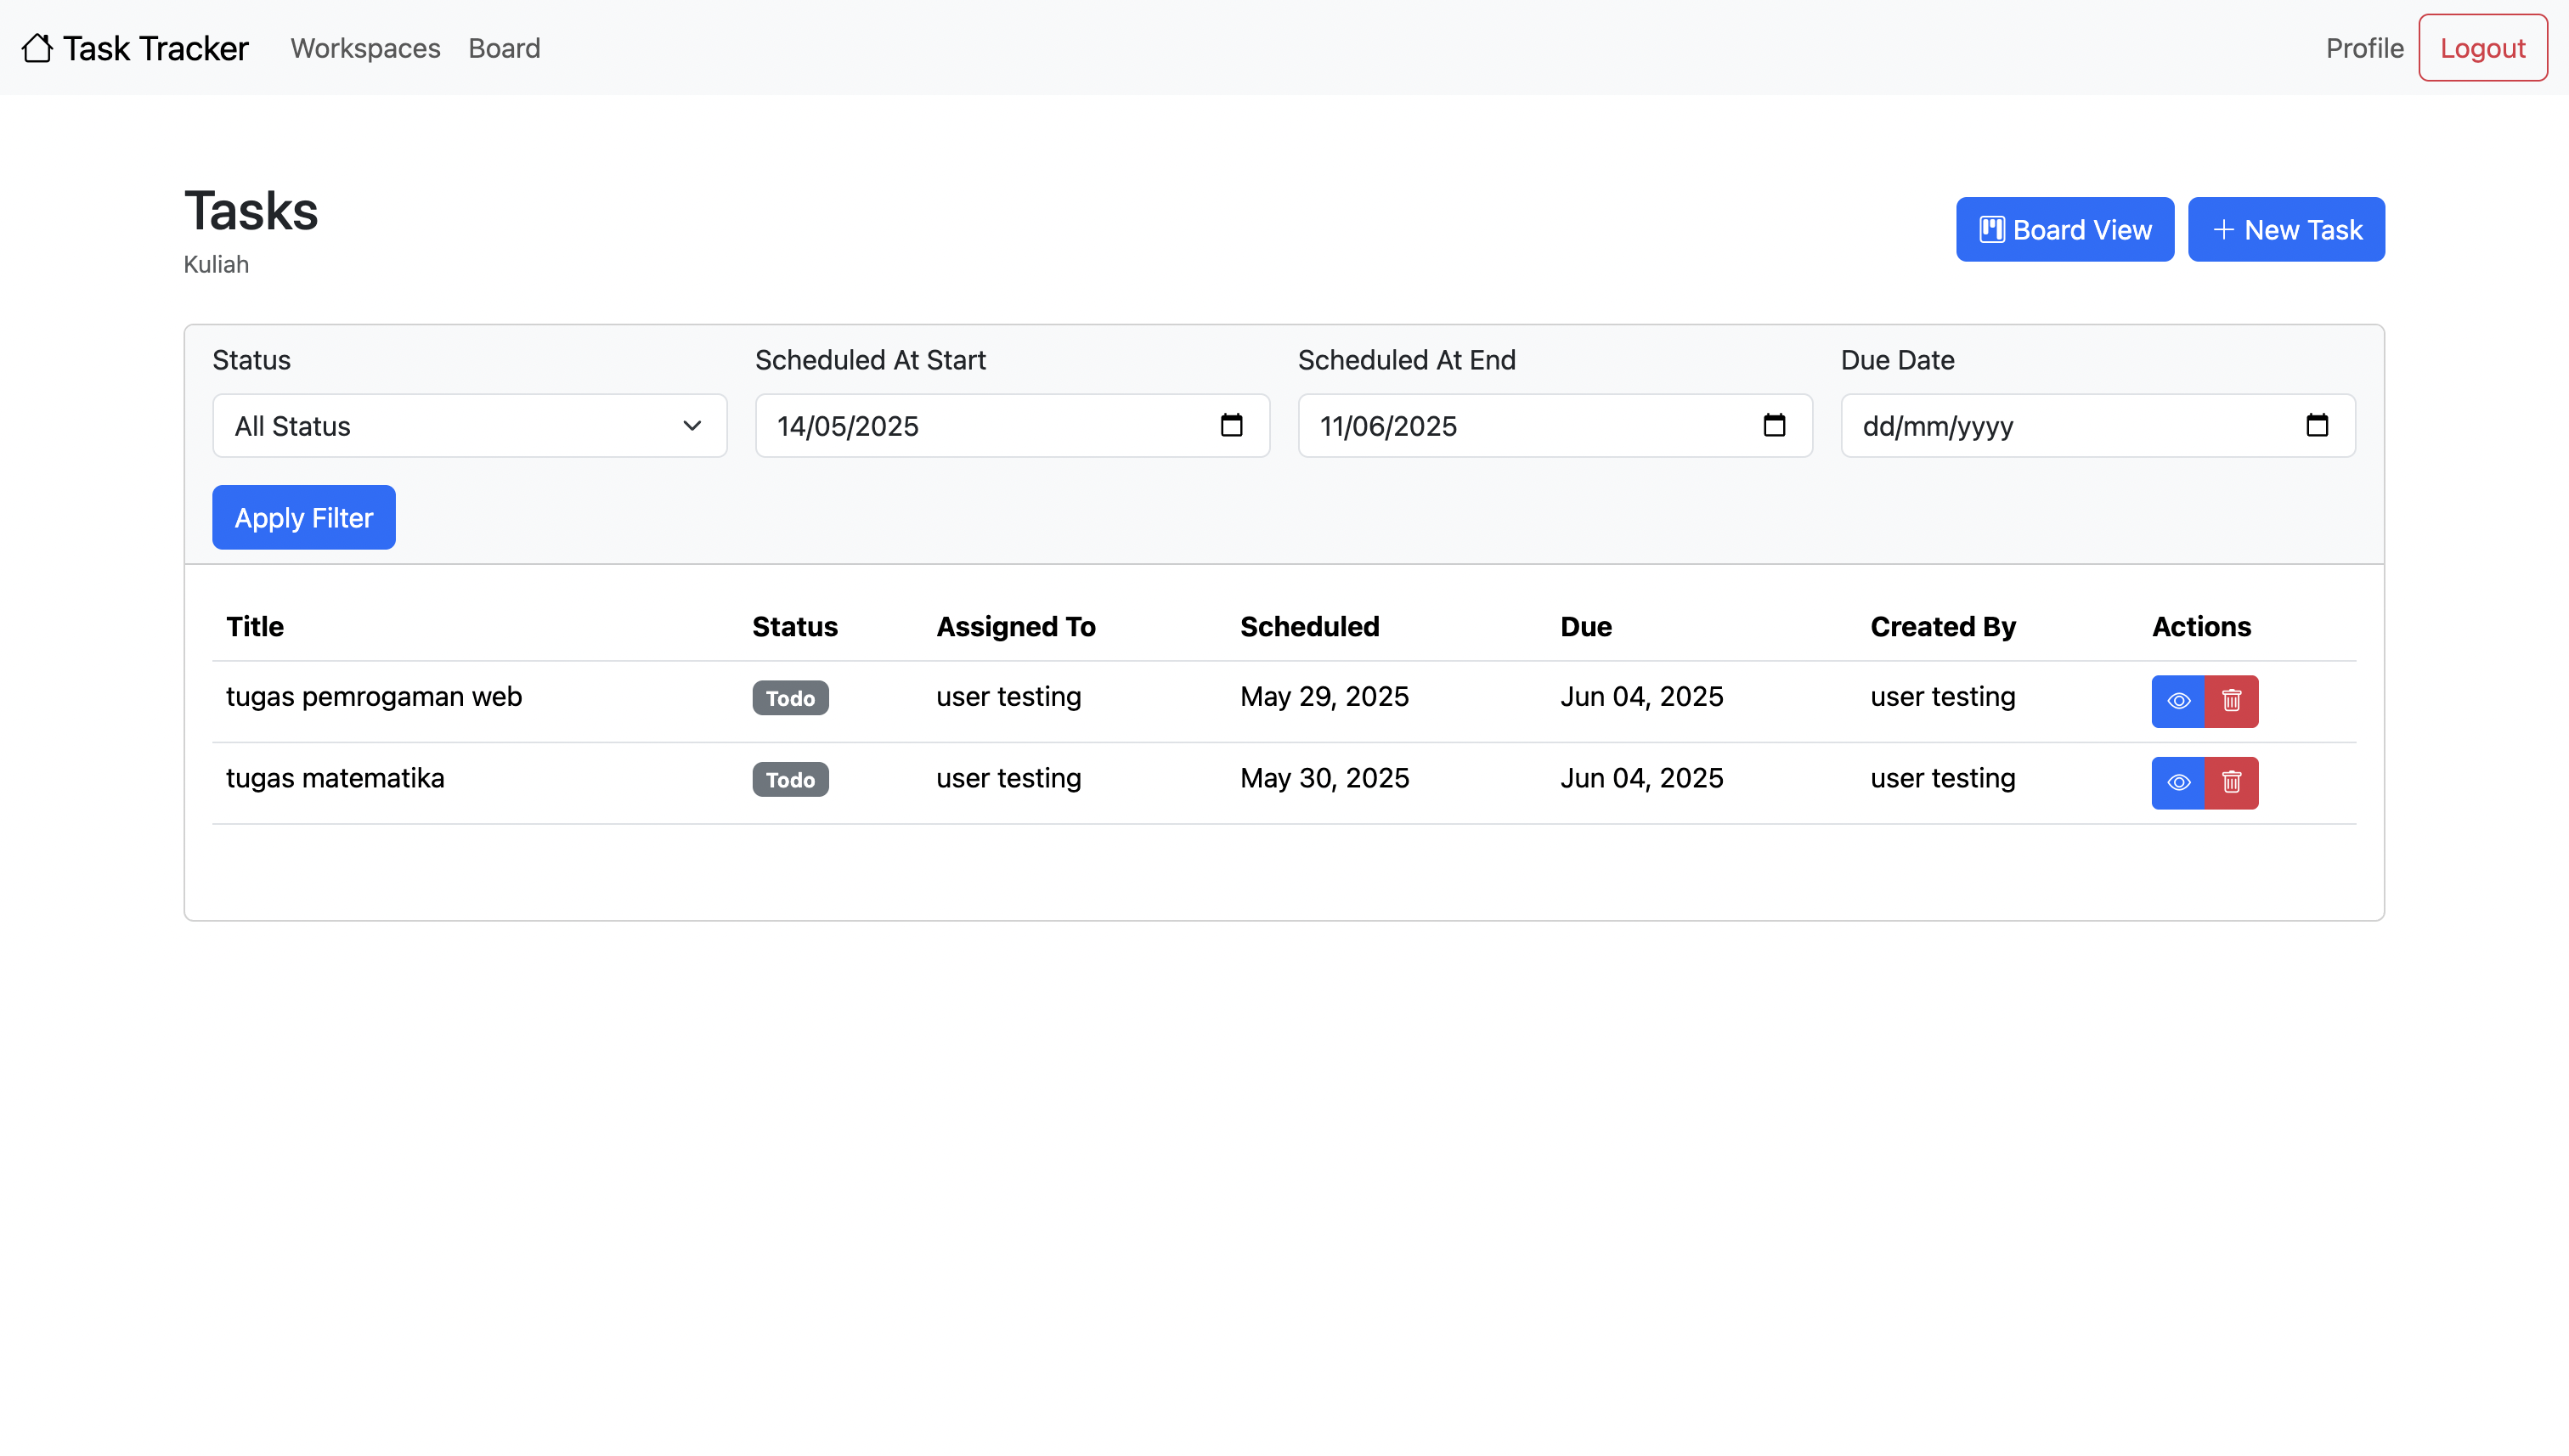
\includegraphics[width=1\textwidth]{assets/ui/list_task.png}
  \captionof{figure}{Tampilan UI List Task}
\end{center}
disini kalian bisa melihat semua task yang ada di dalam workspace.
di pojok kanan atas, terdapat tombol untk kembali ke halaman board, atau untuk membuat task baru,
terdapat juga beberapa filter yang bisa digunakan untuk memfilter task yang ada di dalam list. 
di ui item list task, terdapat beberapa tombol yang bisa digunakan.
\begin{center}
  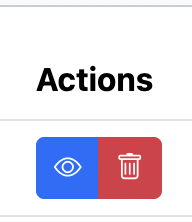
\includegraphics[width=0.3\textwidth]{assets/ui/list_task_action_buttons.png}
  \captionof{figure}{Tampilan Detail Lokasi Tombol Actions}
\end{center}
dari sebelah kiri ke kanan, tombol tersebut adalah:
\begin{itemize}
  \item tombol "mata" digunakan untuk melihat detail task dalam bentuk form yang bisa di edit.
  \item tombol "kotak sampah" digunakan untuk menghapus task.
\end{itemize}
saat klik tombol "mata", maka akan muncul detail task yang ada di dalam task tersebut.
\begin{center}
  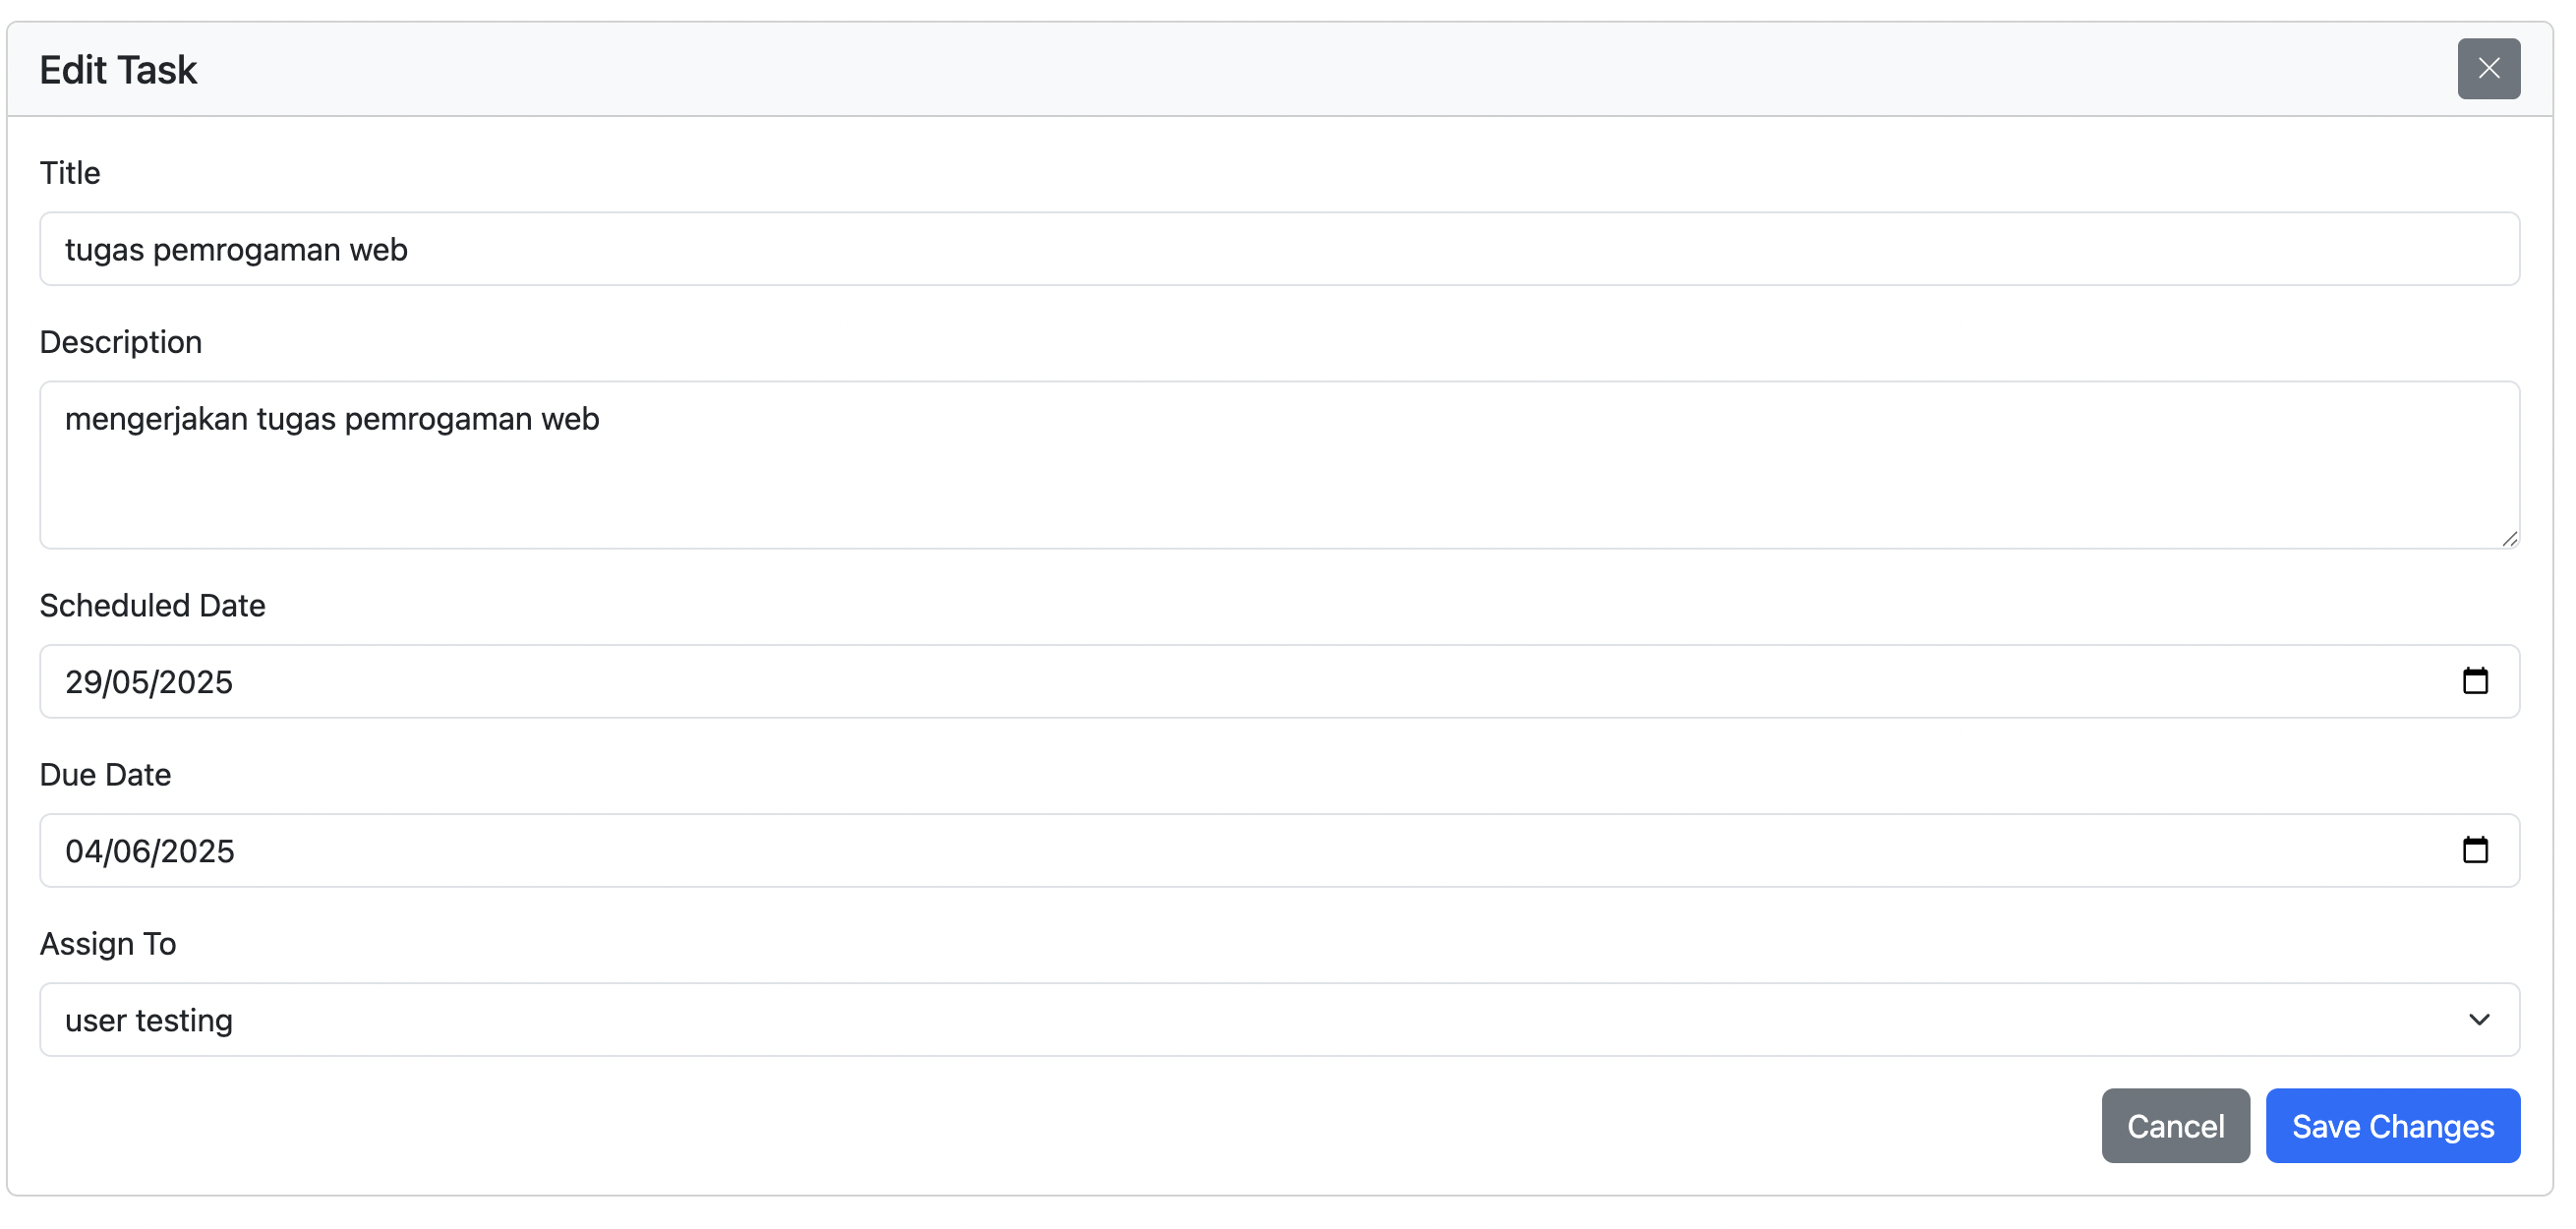
\includegraphics[width=1\textwidth]{assets/ui/list_task_edit.png}
  \captionof{figure}{Tampilan Detail Item Task dengan Form Edit}
\end{center}
di pojok kanan atas, terdapat tombol "+ New Task" untuk membuat task baru.
ketika di klik, maka akan muncul form untuk membuat task baru.
\begin{center}
  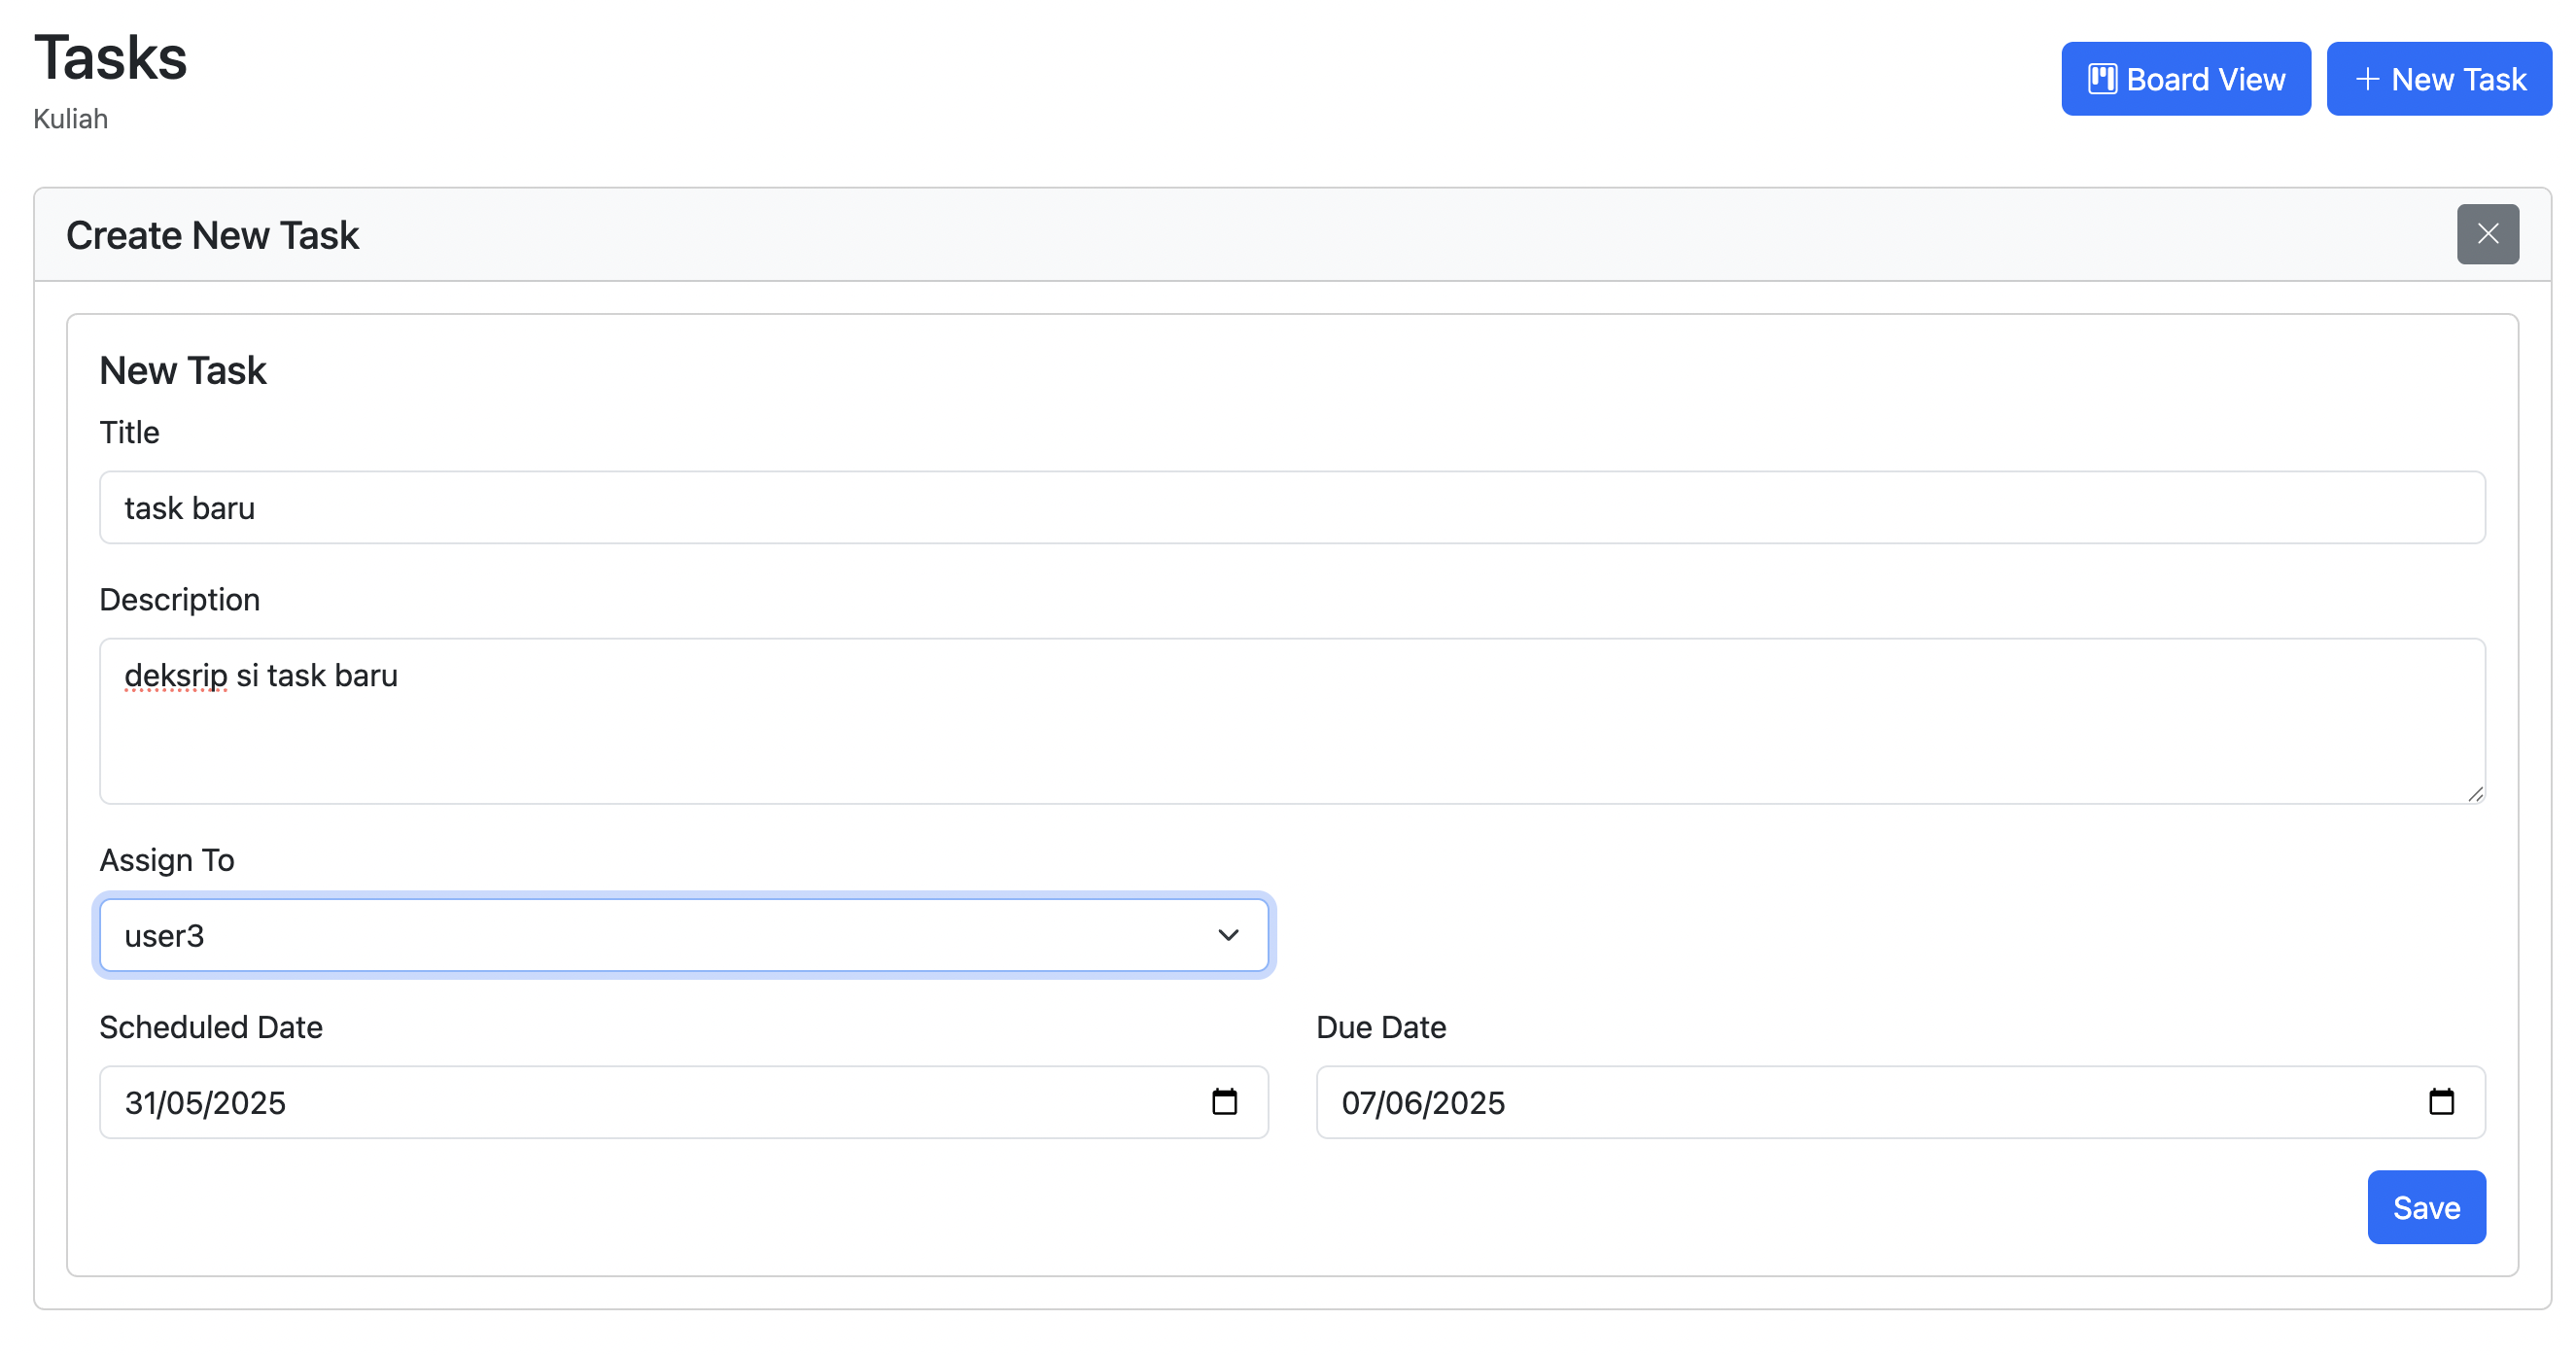
\includegraphics[width=1\textwidth]{assets/ui/list_task_create.png}
  \captionof{figure}{Tampilan UI Form Create Task}
\end{center}








